\section{Режекторная фильтрация: слежение}

\subsection{Анализ системы}

Рассмотрим систему
\begin{equation}
    \label{eq:sys}
    \begin{cases}
        \dot x = Ax+Bu,\\
        y=Cx+Du,
    \end{cases}\quad x(0)=\begin{bmatrix}
        0&0&0
    \end{bmatrix}^T,
\end{equation}
где
\begin{equation*}
    A=\begin{bmatrix}
        3 & 5 & 4 \\
        -2 & -4 & -5 \\
        2 & 2 & 3
    \end{bmatrix},\quad
    B=\begin{bmatrix}
        2 \\ -1 \\ 1
    \end{bmatrix},\quad
    C=\begin{bmatrix}
        -2&-1&0
    \end{bmatrix},\quad
    D=\begin{bmatrix}
        1
    \end{bmatrix},
\end{equation*}
генератор внешнего воздействия
\begin{equation}
    \label{eq:sys_g}
    \begin{cases}
        \dot w_g=\Gamma_gw_g,\\
        g=Y_gw_g,
    \end{cases},\quad w_g(0),
\end{equation}
задающее воздействие $g(t)=8\cos(5t)+2$,  тогда
\begin{equation*}
    \Gamma_g=\begin{bmatrix}
        0 & 5 & 0 \\
        -5& 0 & 0 \\
        0 & 0 & 0
    \end{bmatrix},\quad
    Y_g=\begin{bmatrix}
        8 & 0 & 2
    \end{bmatrix},\quad
    w_g(0)=\begin{bmatrix}
        1 \\ 0 \\ 1
    \end{bmatrix}.
\end{equation*}
внешнее возмущение имеет вид суммы гармоник:
\begin{equation*}
    w_{f_i}(t)=a_i\cos(t)+b_i\sin(t) + c_i\cos(3t)+d_i\sin(3t).
\end{equation*}
Собственные числа матрицы $\Gamma_g$ следующие
\begin{equation}
    \label{eq:specGg}
    \sigma(\Gamma_g)=\{\pm5i,\ 0\}.
\end{equation}
Определим матрицы расширенной модели ошибки
\begin{equation}
    \label{eq:errmodel}
    \dot{\bar e}=\bar A\bar e+\bar Bu+\bar Gg,
\end{equation}
где
\begin{equation*}
    \bar e=\begin{bmatrix}
        e_w\\x
    \end{bmatrix},\quad
    \bar A=\begin{bmatrix}
        \Gamma_g&-GC\\0&A
    \end{bmatrix},\quad
    \bar B=\begin{bmatrix}
        -GD\\B
    \end{bmatrix},\quad
    \bar G=\begin{bmatrix}
        G\\0
    \end{bmatrix},
\end{equation*}
матрицей $G$ зададимся из условия управляемости пары $(\Gamma_g,\ G)$:
\begin{equation*}
    G=\begin{bmatrix}
        1&0&1
    \end{bmatrix}^T.
\end{equation*}
Спектр $\bar A$
\begin{equation}
    \label{eq:abarspec}
    \sigma(A)=\{0,\ 
    \pm 5i,\ 
    2 \pm i,\ 
    -2\}
\end{equation}

\subsection{Без наблюдателя}

\subsubsection{Структурная схема}

Примем вектор состояния $x(t)$ доступным к измерению.
\begin{figure}[H]
    \centering
    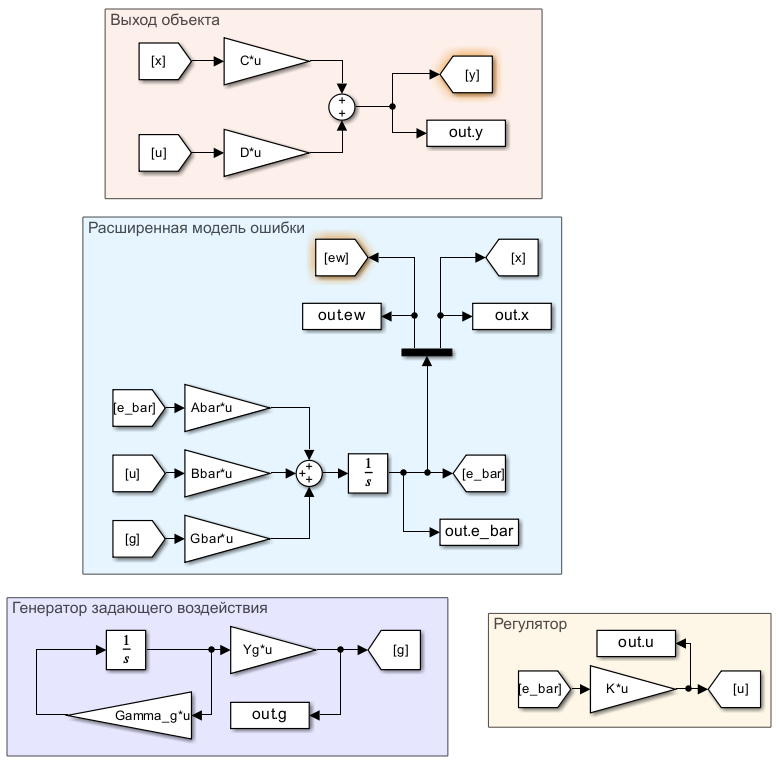
\includegraphics[width=\linewidth]{figs/1_0_slx.png}
    \caption{Структурная схема системы \eqref{eq:sys}, замкнутой регулятором
    \eqref{eq:reg1}}
    \label{fig:1slx}
\end{figure}
Построим схему 
моделирования системы \eqref{eq:sys}, замкнутой регулятором
\begin{equation}
    \label{eq:reg1}
    u=K\bar e,
\end{equation}
обеспечивающим выполнение целевого условия
\begin{equation}
    \label{eq:aim}
    \lim_{t\rightarrow\infty}|\varepsilon|=\lim_{t\rightarrow\infty}|g(t)-y(t)|=0.
\end{equation}
Схему можно увидеть на \autoref{fig:1slx}. 

\subsubsection{Синтез управления}
\label{sec:reg1}

Синтезируем матрицу $K$, для
этого решим уравнение Сильвестра:
\begin{equation}
    \label{eq:silf1}
    \bar AP-P\Gamma=\bar BY,\quad K=-YP^{-1}.
\end{equation}
Для существования решения спеткры $\bar A$ и $\Gamma$ должны не пересекаться, 
пара $(\Gamma,\ Y)$ полностью наблюдаема,
пара $(\bar A,\ \bar B)$ должна быть полностью управляема,
но если посмотреть на матрицы Хаутуса данной пары, собственное число $-2$
окажется неуправляемой, но так как оно меньше нуля, пара стабилизируема.
Тогда сначала усечем систему, жордановы формы матриц:
\begin{equation*}
     \bar A_J=\begin{bmatrix}
        0 & 0 & 0 & 0 & 0 & 0 \\
        0 & -2 & 0 & 0 & 0 & 0 \\
        0 & 0 & 2 & -1 & 0 & 0 \\
        0 & 0 & 1 & 2 & 0 & 0 \\
        0 & 0 & 0 & 0 & 0 & -5 \\
        0 & 0 & 0 & 0 & 5 & 0
        \end{bmatrix},\quad
        B_J=\begin{bmatrix}
        -2.4 \\
        0 \\
        0.7071 \\
        -2.1213 \\
        0.3889 \\
        -0.8485
        \end{bmatrix},
\end{equation*}
\begin{equation*}
    N=\begin{bmatrix}
        0 & 0.069 & -0.0354 & -0.1061 & 0 & 1.4142 \\
        0 & 0.1724 & -0.0354 & 0.2475 & 1.4142 & 0 \\
        1 & 0.5 & 0.2828 & -0.5657 & 0 & 0 \\
        0 & -1 & 0.7071 & -0.7071 & 0 & 0 \\
        0 & 1 & -1.4142 & 0 & 0 & 0 \\
        0 & 0 & 1.4142 & 0 & 0 & 0
        \end{bmatrix},
\end{equation*}
где $N$ - матрица перехода в жордановый базис. Усечем матрицы:
\begin{equation*}
    \bar A_j=\begin{bmatrix}
       0 & 0 & 0 & 0 & 0 \\
       0  & 2 & -1 & 0 & 0 \\
       0  & 1 & 2 & 0 & 0 \\
       0  & 0 & 0 & 0 & -5 \\
       0 & 0 & 0 & 5 & 0
       \end{bmatrix},\quad
       B_j=\begin{bmatrix}
       -2.4 \\
       0.7071 \\
       -2.1213 \\
       0.3889 \\
       -0.8485
       \end{bmatrix},
\end{equation*}
Зададимся матрицами для уравнения Сильвестра:
\begin{equation*}
    \Gamma=\begin{bmatrix}
        -1 & 0 & 0 & 0 & 0 \\
         0 & -3 & 0 & 0 & 0 \\
         0 &  0 & -4 & 0 & 0 \\
         0 &  0 &  0 & -5 & 0 \\
         0 &  0 &  0 &  0 & -6
    \end{bmatrix},\quad
    Y=\begin{bmatrix}
        1 & 1 & 1 & 1 & 1
    \end{bmatrix}.
\end{equation*}
Решив уравнение \eqref{eq:silf1} с помощью CVX, получим
\begin{equation*}
    K_j=\begin{bmatrix}
        1.2000&	-39.5276&	0.9192	&-6.5425&	-14.5249
    \end{bmatrix},
\end{equation*}
вернем прежний размер
\begin{equation*}
    K_J=\begin{bmatrix}
        1.2000	&0 &-39.5276	&0.9192	&-6.5425	&-14.5249
    \end{bmatrix}
\end{equation*}
и переведем в изначальный базис
\begin{equation*}
    K=K_JN^{-1}=\begin{bmatrix}
        -10.2706	&-4.6262&	1.2000&	-2.3386&	-1.4326&	-28.8260
    \end{bmatrix}.
\end{equation*}
Проверим, что получился желаемый спектр:
\begin{equation*}
    \sigma(\bar A+\bar BK)=\{-5.9692,\ -5.0652
    -3.9539,\ 
    -3.0119,\ 
    -0.9999,\ 
    -2.0000\}.
\end{equation*}
Как видно, желаемый спектр получем, но с небольшой погрешностью.

\subsubsection{Передаточная функция}

Определим ПФ от задающего воздействия к ошибке слежения:
\begin{equation*}
    \underset{g\rightarrow\varepsilon}{W}=-\bar C(sI-(\bar A+\bar BK))^{-1}\bar G+1,
\end{equation*}
где $\bar C=[0\quad C] + DK$, с помощью MATLAB получим
\begin{equation*}
    \underset{g\rightarrow\varepsilon}{W}=\frac{s\,{\left(\text{2.535e+30}\,s^4 +\text{7.117e+31}\,s^3 +\text{1.277e+32}\,s^2 +\text{1.779e+33}\,s+\text{1.608e+33}\right)}}{\text{2.535e+30}\,s^5 +\text{4.817e+31}\,s^4 +\text{3.473e+32}\,s^3 +\text{1.169e+33}\,s^2 +\text{1.78e+33}\,s+\text{9.127e+32}}.
\end{equation*}
Данная ПФ имеет нули $\left(\begin{array}{c}
0\\
-27.14\\
-0.9352\\
-5.0\,\mathrm{i}\\
5.0\,\mathrm{i}
\end{array}\right)$ и полюса $\left(\begin{array}{c}
-0.9999\\
-3.012\\
-3.954\\
-5.065\\
-5.969
\end{array}\right)$, как видно, нули содержат спектр задающего воздействия, что 
соответствует принципу внутренней модели, которым мы руководствовались, а полюса
содержат динамику замкнутой системы, которую задали матрицей $\Gamma$. 
Проверим выполнение целевого условия \eqref{eq:aim}, используя теорему о предельном
значении:
\begin{multline*}
    \lim_{t\rightarrow\infty}|\varepsilon(t)|=\lim_{s\rightarrow0}|sE(s)|=
    \lim_{s\rightarrow0}|s\underset{g\rightarrow\varepsilon}{W}(s)G(s)|=
    \lim_{s\rightarrow0}|s\underset{g\rightarrow\varepsilon}{W}(s)(Y_g(sI-\Gamma_g)^{-1}w_{g}(0))|=\\
    \hspace*{-1.5cm}\lim_{s\rightarrow0}\Big|s\frac{10.0\,{\left(s^2 +5.0\right)}\,{\left(\text{2.535e+30}\,s^4 +\text{7.117e+31}\,s^3 +\text{1.277e+32}\,s^2 +\text{1.779e+33}\,s+\text{1.608e+33}\right)}}{{\left(s^2 +25.0\right)}\,{\left(\text{2.535e+30}\,s^5 +\text{4.817e+31}\,s^4 +\text{3.473e+32}\,s^3 +\text{1.169e+33}\,s^2 +\text{1.78e+33}\,s+\text{9.127e+32}\right)}}\Big|=0.
\end{multline*}
Условие выполняется.

\subsubsection{Моделирование}

Выполним компьютерное моделирование системы, замкнутой регулятором
\eqref{eq:reg1} и построим графики задающего воздействия $g(t)$, формируемого 
регулятором управления $u(t)$, вектора состояния замкнутой системы $x(t)$, выхода
$y(t)$ и ошибки регулирования $\varepsilon(t) = g(t) - y(t)$. Графики можно
увидеть на рисунке \ref{fig:1_0_sim}.

\begin{figure}[H]
    \centering
    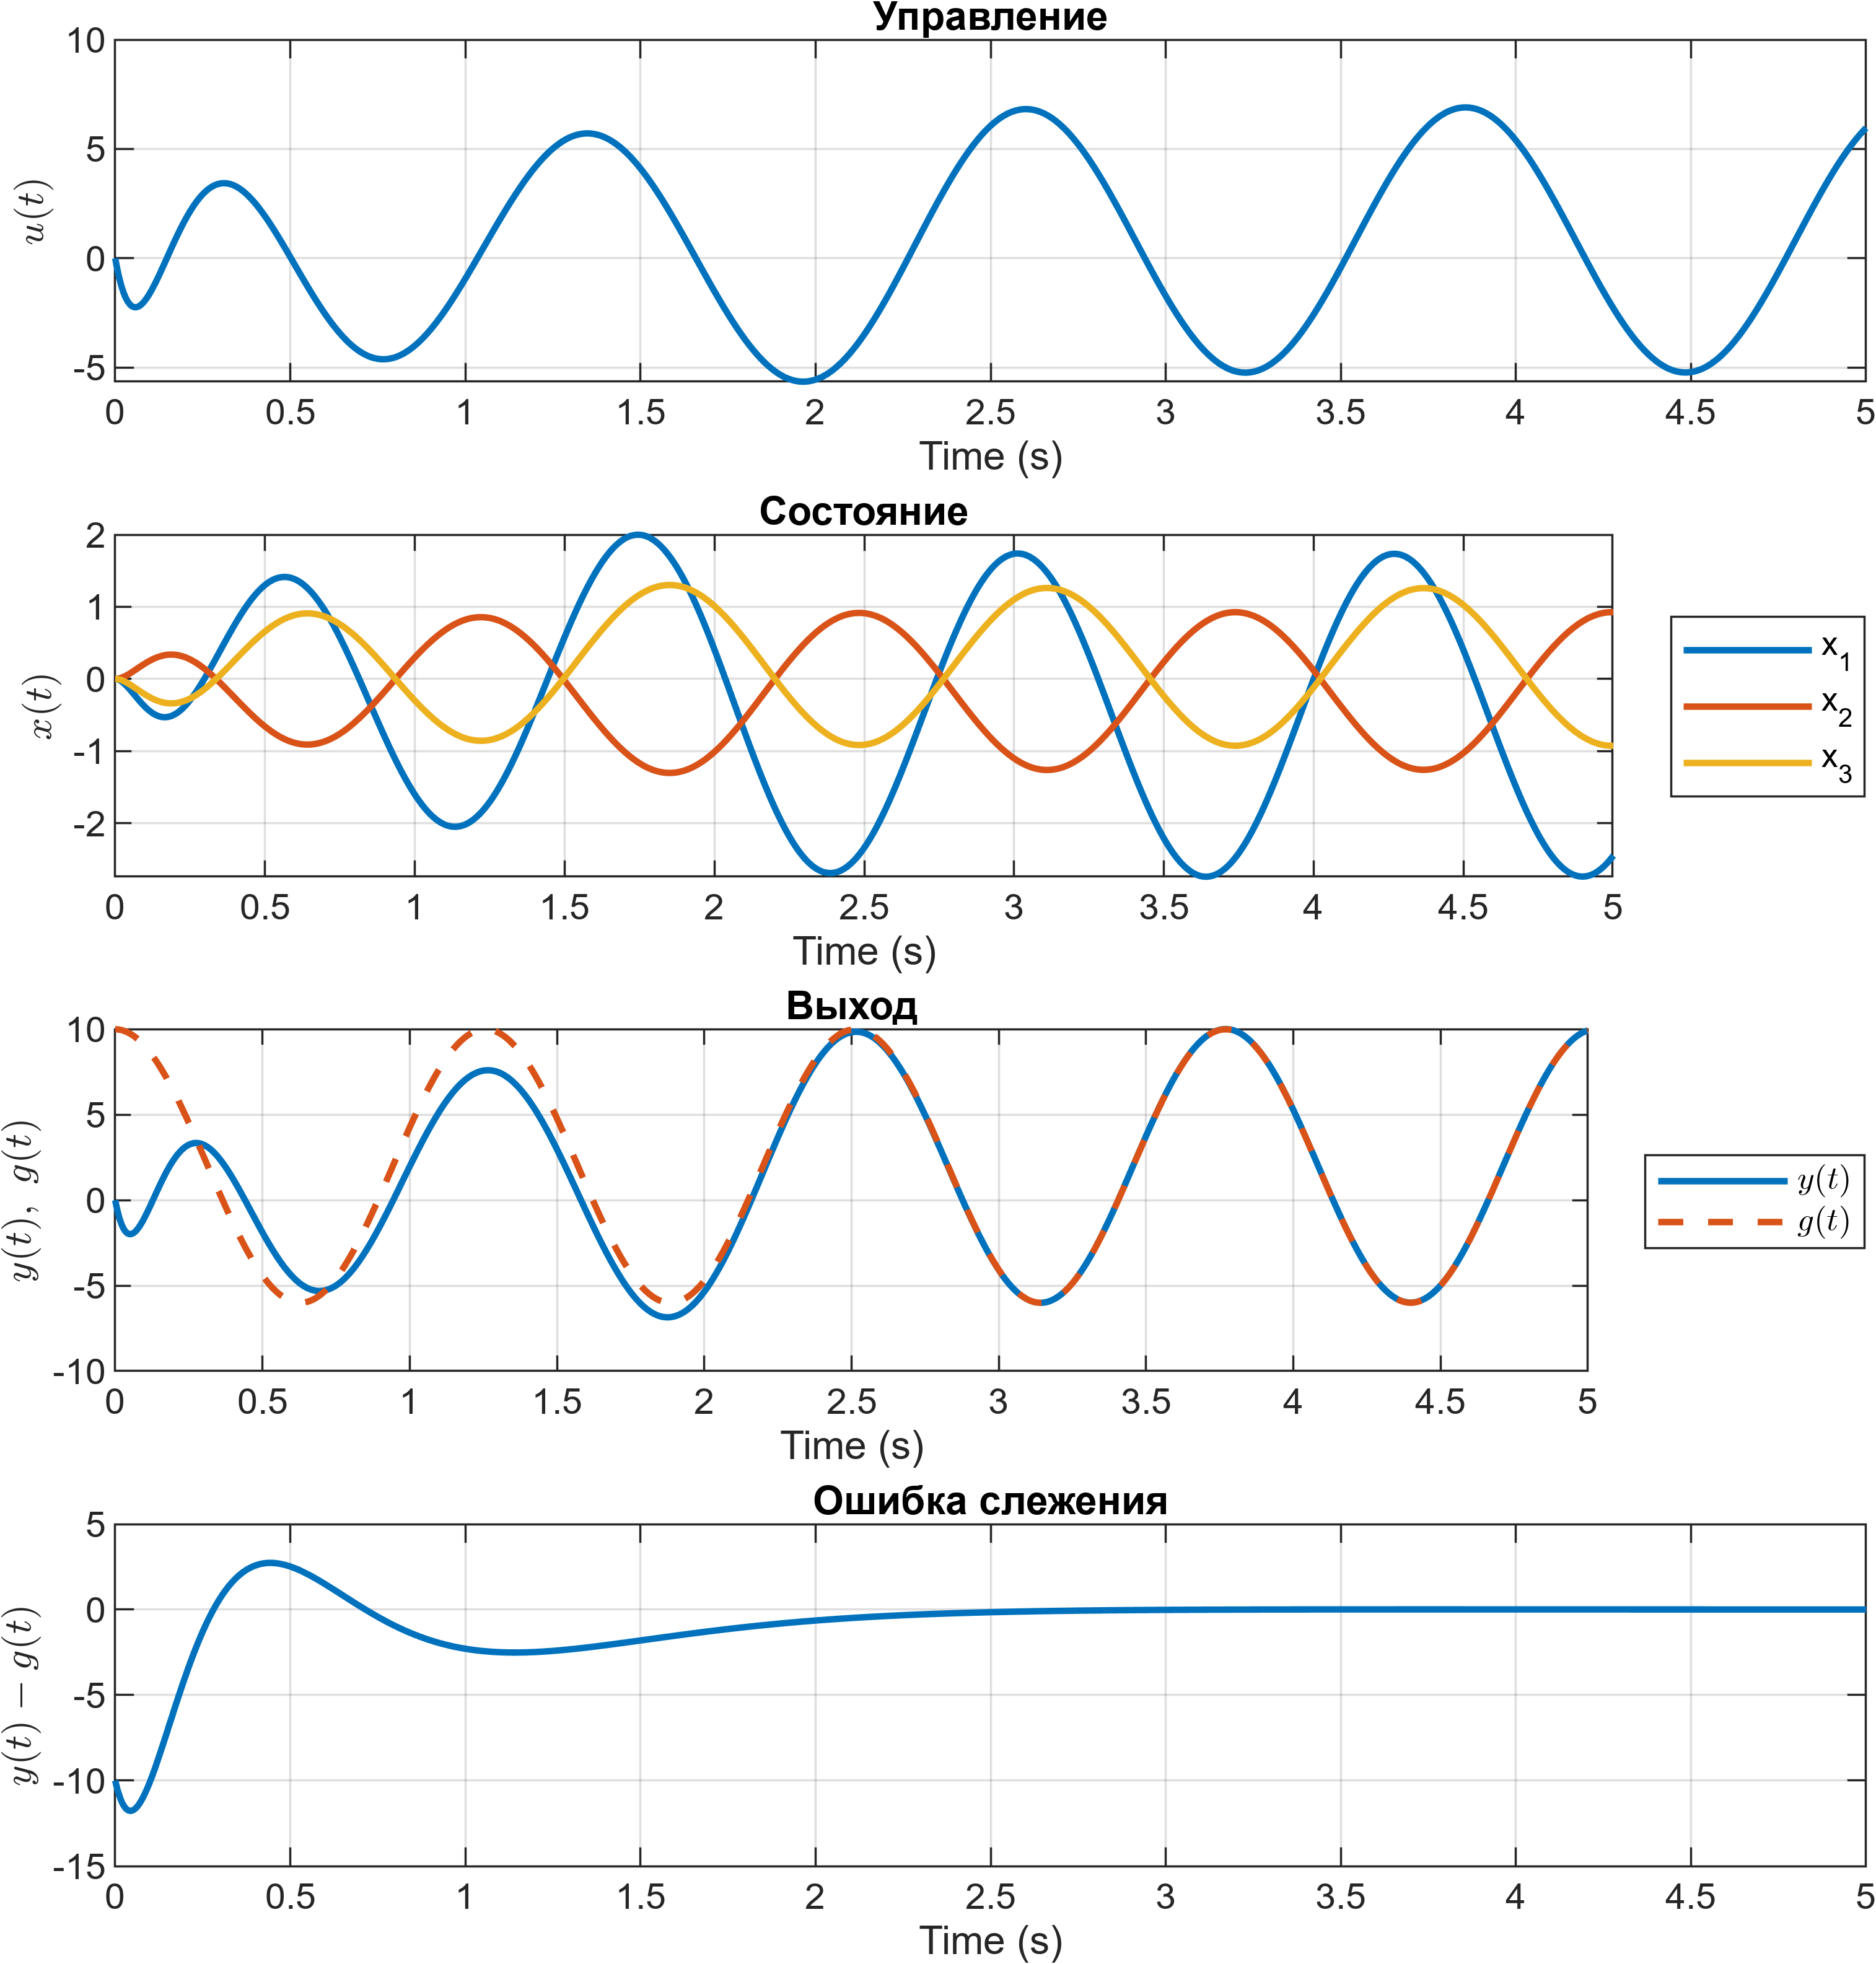
\includegraphics[width=\linewidth]{figs/1_0_sim.png}
    \caption{Графики задающего воздействия $g(t)$, выхода
    $y(t)$, ошибки регулирования $\varepsilon(t) = g(t) - y(t)$,
    управления $u(t)$ и вектора состояния замкнутой системы $x(t)$}
    \label{fig:1_0_sim}
\end{figure}



\subsection{С наблюдателем}

\subsubsection{Структурная схема}

Примем вектор состояния $x(t)$ недоступным к измерению. Значит придется 
"прикрутить" наблюдатель:
\begin{equation}
    \label{eq:obs1}
    \begin{cases}
        \dot{\hat x}=A\hat x+Bu+L(\hat y - y),\\
        \hat y=C\hat x+Du.
    \end{cases}
\end{equation}
\begin{figure}[H]
    \centering
    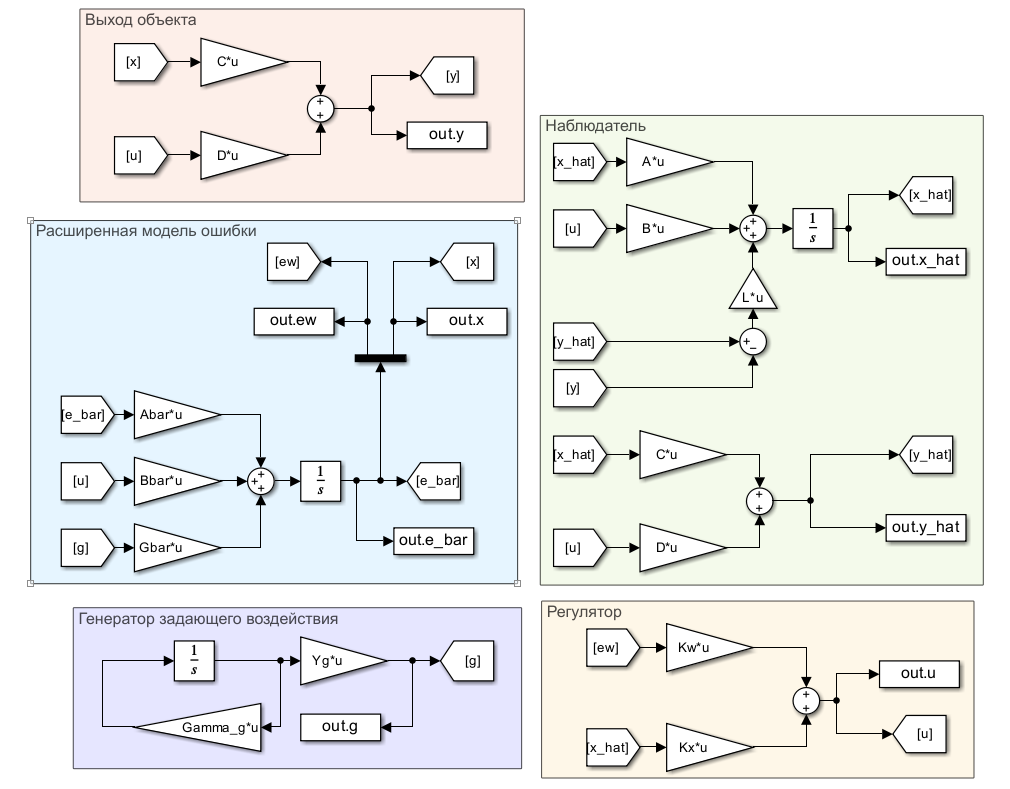
\includegraphics[width=\linewidth]{figs/1_1_slx.png}
    \caption{Структурная схема системы \eqref{eq:sys}, замкнутой регулятором
    \eqref{eq:reg11}}
    \label{fig:11slx}
\end{figure}
\noindent Построим схему моделирования системы \eqref{eq:sys}, замкнутой регулятором
\begin{equation}
    \label{eq:reg11}
    u=K_we_w+K_x\hat x
\end{equation}
с наблюдателем \eqref{eq:obs1},
обеспечивающим выполнение целевого условия \eqref{eq:aim}. Матрицы $K_w$, $K_x$
берем из $K$ \autoref{sec:reg1}:
\begin{equation*}
    K=\begin{bmatrix}
        K_w & K_x
    \end{bmatrix}.
\end{equation*}
Схему можно увидеть на \autoref{fig:11slx}. 

\subsubsection{Синтез наблюдателя}
\label{eq:obs}

Для синтеза наблюдателя \eqref{eq:obs1} найдем матрицу $L$ с помощью уравнения Сильвестра:
\begin{equation*}
    QA-\Gamma Q=YC,\quad L=-Q^{-1}Y.
\end{equation*}
Для существования решения спектры $A$ и $\Gamma$ должны не пересекаться, пара $(C,\ A)$
наблюдаема, в чем можно убедиться с помощью матрицы наблюдаемости, и пара $(\Gamma,\ Y)$ 
управляема. Матриц $A$ имеет спектр $\{2 \pm i,\ -2\}$. Тогда пусть
\begin{equation*}
    \Gamma=\begin{bmatrix}
        -3 & 0 & 0\\
        0 & -4 & 0\\
        0 & 0 & -5
    \end{bmatrix},\quad
    Y=\begin{bmatrix}
        1\\1\\1
    \end{bmatrix}.
\end{equation*}
С помощью CVX получим
\begin{equation*}
    L=\begin{bmatrix}
        -18.5294&51.0588&-51.4118
    \end{bmatrix}^T.
\end{equation*}

\subsubsection{Передаточная функция}

Определим ПФ от задающего воздействия к ошибке слежения. Для этого определим новую 
внутренную модель ошибки слежения:
\begin{equation*}
    \begin{cases}
        \dot e_w=\Gamma_ge_w+G(g-\hat y)\\
        \dot x=Ax+Bu\\
        \dot{\hat x}=A\hat x+Bu+L(\hat y - y)
    \end{cases}\Rightarrow
    \begin{cases}
        \dot e_w=\Gamma_ge_w-GC\hat x-GDu+Gg\\
        \dot x=Ax+Bu\\
        \dot{\hat x}=-LCx+(A+LC)\hat x+Bu
    \end{cases}
\end{equation*}
Определим новую систему
\begin{equation*}
    \dot{\tilde e}=\tilde A\tilde e+\tilde B u+\tilde Gg,
\end{equation*}
где
\begin{equation*}
    \tilde e=\begin{bmatrix}
        e_w\\x\\ \hat x
    \end{bmatrix},\quad
    \tilde A=\begin{bmatrix}
        \Gamma&0&-GC\\0&A&0\\0&-LC&A+LC
    \end{bmatrix},\quad
    \tilde B=\begin{bmatrix}
        -GC\\B\\B
    \end{bmatrix},\quad
    \tilde G=\begin{bmatrix}
        G\\0
    \end{bmatrix}.
\end{equation*}
Добавим выход:
\begin{equation*}
    \begin{cases}
        \dot{\tilde e}=\tilde A\tilde e+\tilde B u+\tilde Gg\\
        \varepsilon=g-\tilde C\tilde e
    \end{cases},\quad
    \tilde C=\begin{bmatrix}
        DK_w&0&C+DK_x
    \end{bmatrix}.
\end{equation*}
Переопределим матрицу $K$:
\begin{equation*}
    K=\begin{bmatrix}
        K_w&0&K_x
    \end{bmatrix}
\end{equation*}
Проверим замкнутую систему:
\begin{equation*}
    \sigma(\tilde A+\tilde B\tilde K)=\left(\begin{array}{c}
-5.969\\
-0.9999\\
-5.065\\
-3.954\\
-5.0\\
-4.0\\
-3.012\\
-3.0\\
-2.0
\end{array}\right),
\end{equation*}
как видно, замкнутая система устойчива и содержит спектр наблюдателя $A+LC$, желаемый спеткр замкнутой системы $\Gamma$
и неуправляемое собственное число $-2$.
Формула ПФ:
\begin{equation*}
    \underset{g\rightarrow\varepsilon}{W}=\tilde C(sI-(\tilde A+\tilde BK))^{-1}\tilde G+1,
\end{equation*}
с помощью MATLAB получим
\begin{equation*}
    \underset{g\rightarrow\varepsilon}{W}=\frac{s\,{\left(6.066\,s^7 + 243.1\,s^6 + 2634\,s^5 + 16290\,s^4 + 79510\,s^3 + 264600\,s^2 + 436300\,s + 230900\right)}}{6.066\,s^8 + 188\,s^7 + 2499\,s^6 + 18550\,s^5 + 83790\,s^4 + 234600\,s^3 + 394100\,s^2 + 358100\,s + 131000}.
\end{equation*}
Данная ПФ имеет нули $\left(\begin{array}{c}
0\\
-5.0\,\mathrm{i}\\
5.0\,\mathrm{i}\\
-0.9352\\
-3.0\\
-4.0\\
-5.0\\
-27.14
\end{array}\right)$ и полюса $\left(\begin{array}{c}
-0.9999\\
-3.0\\
-3.012\\
-3.954\\
-4.0\\
-5.0\\
-5.065\\
-5.969
\end{array}\right)$, как видно, нули содержат спектр задающего воздействия, что 
соответствует принципу внутренней модели, которым мы руководствовались, этот же спектр 
содержит нули ПФ для случая без наблюдателя и 
дополнительно спектр наблюдателя ($A+LC$); полюса так же содержат полюса ПФ случая без
наблюдателя и дополнительно спектр наблюдателя ($A+LC$).
Проверим выполнение целевого условия \eqref{eq:aim}, используя теорему о предельном
значении:
\begin{multline*}
    \lim_{t\rightarrow\infty}|\varepsilon(t)|=\lim_{s\rightarrow0}|sE(s)|=
        \lim_{s\rightarrow0}|s\underset{g\rightarrow\varepsilon}{W}(s)G(s)|=
        \lim_{s\rightarrow0}|s\underset{g\rightarrow\varepsilon}{W}(s)(Y_g(sI-\Gamma_g)^{-1}w_{g}(0))|=\\
            \hspace*{-1.5cm}\lim_{s\rightarrow0}\Big|s\frac{10.0\,{\left(s^2 +5.0\right)}\,{\left(0.06066\,s^7 +2.431\,s^6 +26.34\,s^5 +162.9\,s^4 +795.1\,s^3 +2646\,s^2 +4363\,s+2309\right)}}{{\left(s^2 +25.0\right)}\,{\left(0.06066\,s^8 +1.88\,s^7 +24.99\,s^6 +185.5\,s^5 +837.9\,s^4 +2346\,s^3 +3941\,s^2 +3581\,s+1310\right)}}\Big|=0.
        \end{multline*}
Условие выполняется.

\subsubsection{Моделирование}

Выполним компьютерное моделирование системы, замкнутой регулятором
\eqref{eq:reg11} и наблюдателем \eqref{eq:obs1} с единичными начальными условиями, 
и построим графики задающего воздействия $g(t)$, формируемого 
регулятором управления $u(t)$, вектора состояния замкнутой системы $x(t)$, его оценки и их разности, выхода
$y(t)$ и ошибки регулирования $\varepsilon(t) = g(t) - y(t)$. Графики можно
увидеть на рисунках \ref{fig:1_1_0_sim} и \ref{fig:1_1_1_sim}.

\begin{figure}[H]
    \centering
    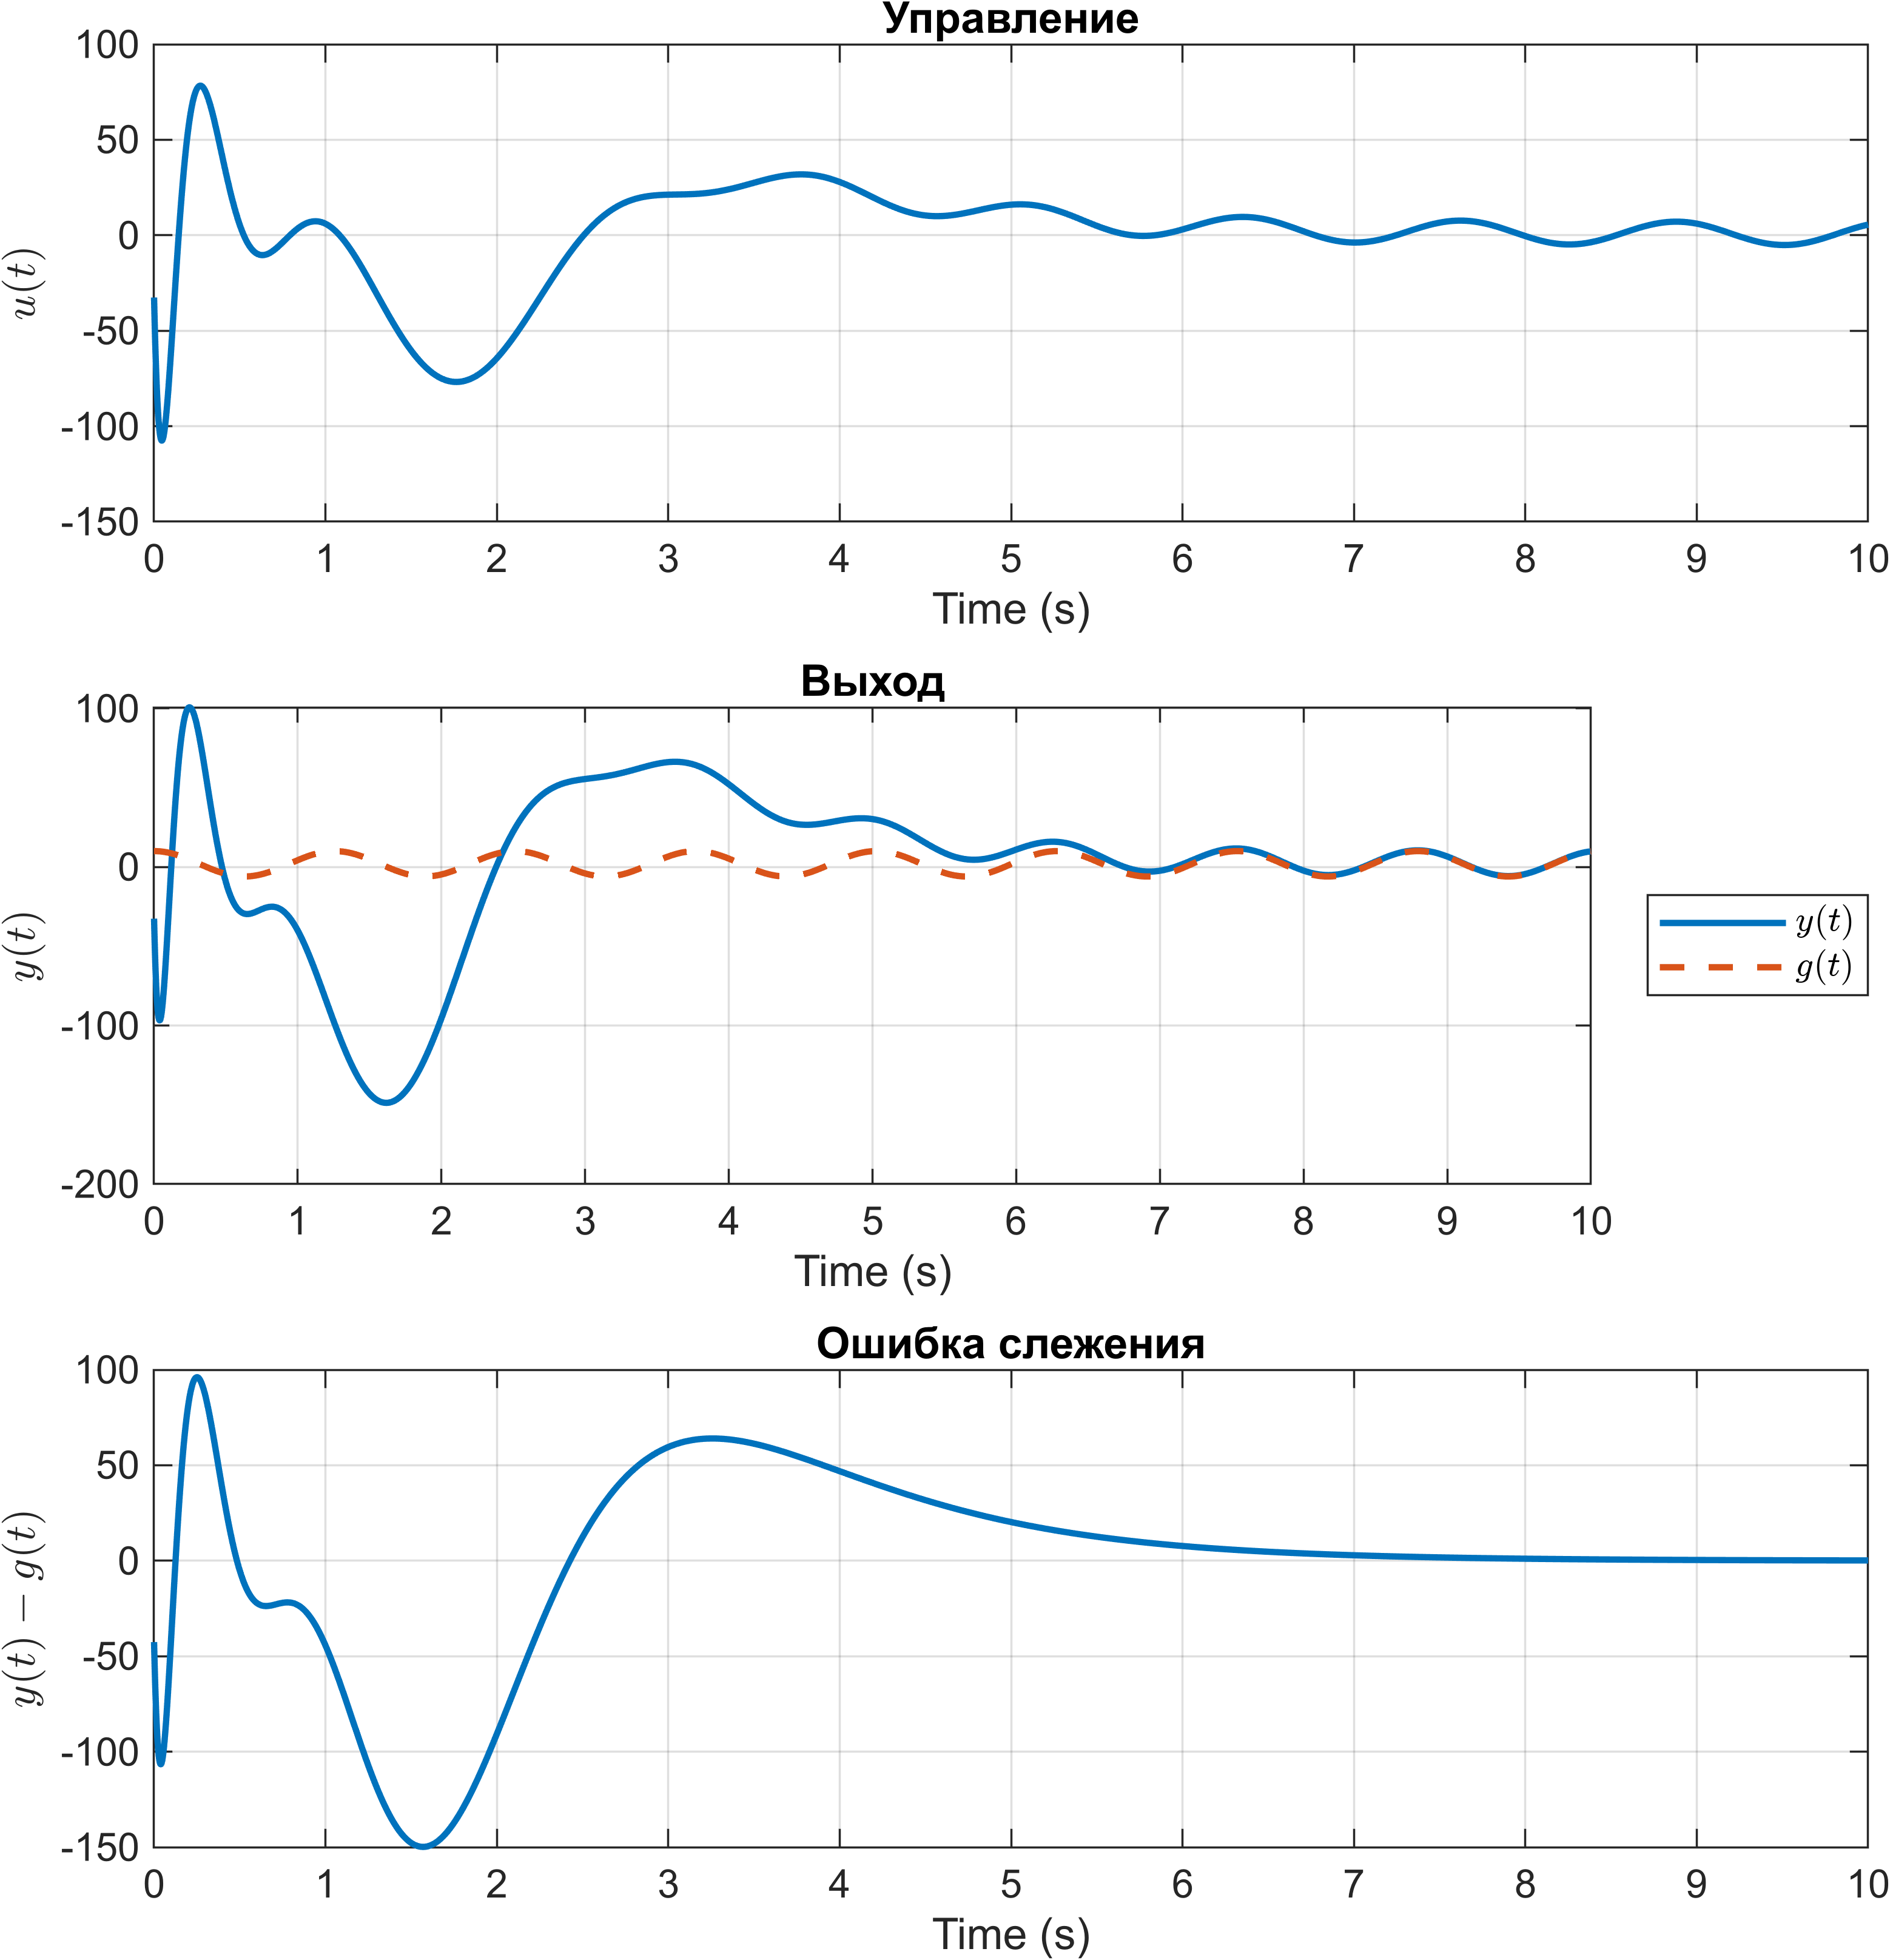
\includegraphics[width=\linewidth]{figs/1_1_0_sim.png}
    \caption{Графики задающего воздействия $g(t)$, выхода
    $y(t)$, ошибки регулирования $\varepsilon(t) = g(t) - y(t)$,
    управления $u(t)$}
    \label{fig:1_1_0_sim}
\end{figure}

\begin{figure}[H]
    \centering
    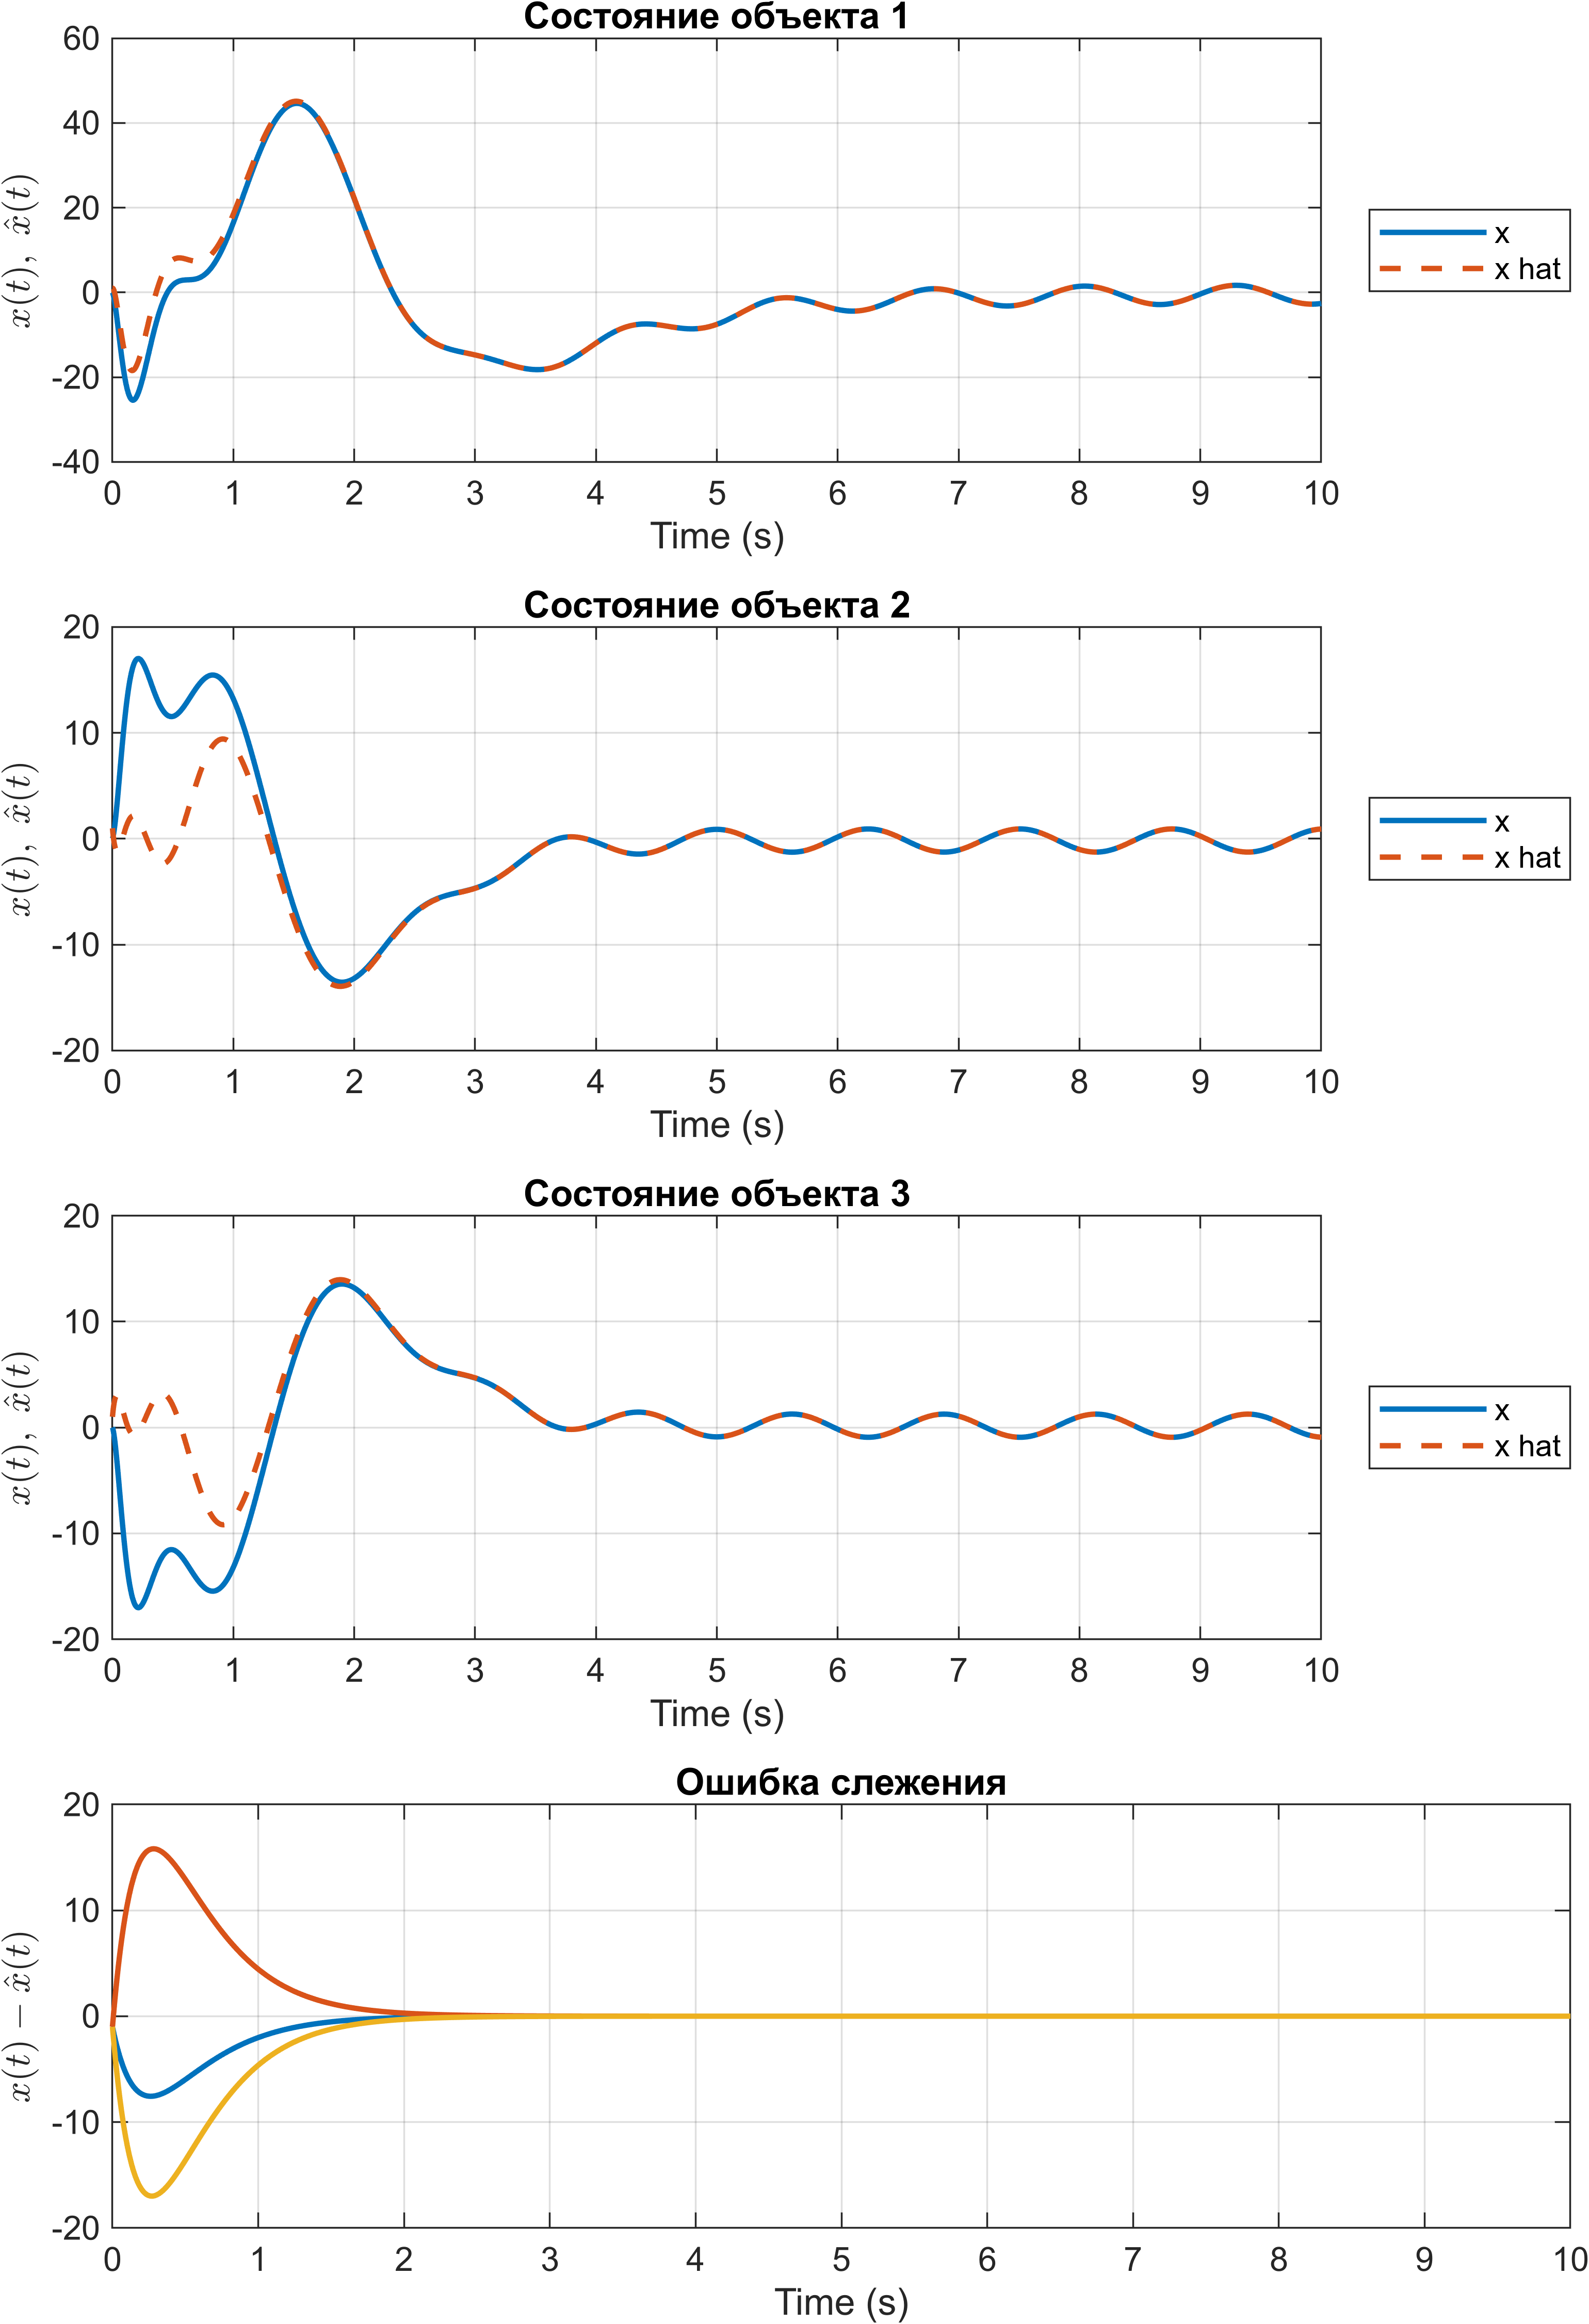
\includegraphics[width=\linewidth]{figs/1_1_1_sim.png}
    \caption{Графики вектора состояния замкнутой системы $x(t)$, его оценки наблюдателем и 
    их разности}
    \label{fig:1_1_1_sim}
\end{figure}


\subsection{Выводы}

Было рассмотрено слежение за сигналом с помощью режекторной фильтрации с и без наблюдателя.
В обоих случаях выполняется принцип внутренней модели, то есть в ПФ от задающего сигнала 
к ошибке между им и выходом системы содержится спектр задающего воздействия. Моделирование показало,
что в обоих случаях система успешно следила за сигналом. Ожидаемо, система без наблюдателя
сходится быстрее, в случае с наблюдателем $y$ сходится к $g$ где-то за 8 секунд, а 
в случае без наблюдателя - за примерно 3 секунды, что можно объяснить тем, что системе сначала
требуется, чтобы наблюдатель состояния сошелся.





\section{Режекторная фильтрация: компенсация}

\subsection{Анализ системы}

Рассмотрим систему
\begin{equation}
    \label{eq:sys1}
    \begin{cases}
        \dot x = Ax+Bu+B_ff,\\
        y=Cx+Du+D_ff,
    \end{cases}\quad x(0)=\begin{bmatrix}
        0&0&0
    \end{bmatrix}^T,
\end{equation}
где
\begin{equation*}
    A=\begin{bmatrix}
        3 & 5 & 4 \\
        -2 & -4 & -5 \\
        2 & 2 & 3
    \end{bmatrix},\quad
    B=\begin{bmatrix}
        2 \\ -1 \\ 1
    \end{bmatrix},\quad
    B_f=\begin{bmatrix}
        -2 & 2 \\ -2 & 0 \\ 0 & 0
    \end{bmatrix},
\end{equation*}
\begin{equation*}
    C=\begin{bmatrix}
        -2&-1&0
    \end{bmatrix},\quad
    D=\begin{bmatrix}
        1
    \end{bmatrix},\quad
    D_f=\begin{bmatrix}
        4&1
    \end{bmatrix},
\end{equation*}
генератор внешнего воздействия
\begin{equation}
    \label{eq:sys_f}
    \begin{cases}
        \dot w_f=\Gamma_fw_f,\\
        f=Y_fw_f,
    \end{cases},\quad     w_f(0)=\begin{bmatrix}
        1&1&1&1
    \end{bmatrix}^T,
\end{equation}
где
\begin{equation*}
    \Gamma_f=\begin{bmatrix}
        35& 56& 22& -42\\
        -11& -17& -7& 12\\
        -6& -10& -5& 10\\
        11 &18& 6& -13
    \end{bmatrix},\quad
    Y_f=\begin{bmatrix}
        1&3\\2&4\\1&2\\-1&-3
    \end{bmatrix}^T.
\end{equation*}
Собственные числа матрицы $\Gamma_f$ следующие
\begin{equation}
    \label{eq:specGf}
    \sigma(\Gamma_f)=\{\pm3i,\ \pm i\},
\end{equation}
внешнее возмущение имеет вид суммы гармоник:
\begin{equation*}
    w_{f_i}(t)=a_i\cos(t)+b_i\sin(t) + c_i\cos(3t)+d_i\sin(3t).
\end{equation*}
Определим матрицы расширенной модели ошибки
\begin{equation*}
    \dot{\bar x}=\bar A\bar x+\bar Bu+\bar B_ff,
\end{equation*}
зададимся матрицей $G$ исходя из условия управляемости пары $(\Gamma_f,\ G)$:
\begin{equation*}
    G=\begin{bmatrix}
        1&1&1&1
    \end{bmatrix}^T,
\end{equation*}
\begin{equation*}
    \bar A=\begin{bmatrix}
        \Gamma_f &GC\\ 0& A
    \end{bmatrix},\quad
    \bar B = \begin{bmatrix}
        GD\\ B
    \end{bmatrix},\quad
    \bar B_f=\begin{bmatrix}
        GD_f\\B_f
    \end{bmatrix}.
\end{equation*}
Спектр матрицы $\bar A$:
\begin{equation*}
    \sigma(A)=\{\pm 3i,\ 
    \pm i,\ 
    2 \pm i,\ 
    -2\}.
\end{equation*}


\subsection{Без наблюдателя}

\subsubsection{Структурная схема}

Примем вектор состояния $x(t)$ доступным к измерению.
\begin{figure}[H]
    \centering
    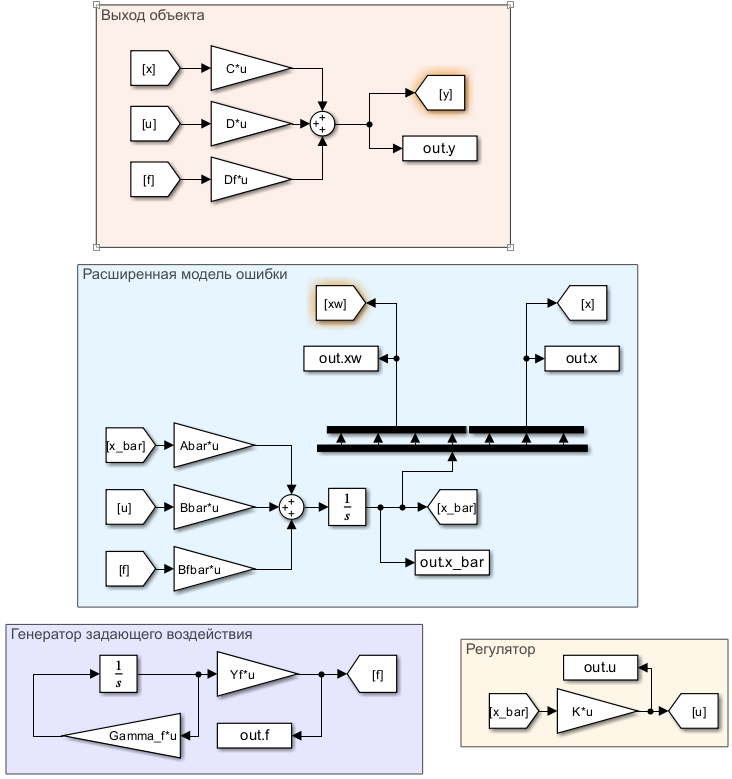
\includegraphics[width=\linewidth]{figs/2_0_slx.png}
    \caption{Структурная схема системы \eqref{eq:sys1}, замкнутой регулятором
    \eqref{eq:reg2}}
    \label{fig:20slx}
\end{figure}
Построим схему 
моделирования системы \eqref{eq:sys1}, замкнутой регулятором
\begin{equation}
    \label{eq:reg2}
    u=K\bar x,
\end{equation}
обеспечивающим выполнение целевого условия
\begin{equation}
    \label{eq:aim2}
    \lim_{t\rightarrow\infty}|y(t)|=0.
\end{equation}
Схему можно увидеть на \autoref{fig:20slx}. 

\subsubsection{Синтез управления}
\label{sec:reg2}

Синтезируем матрицу $K$, для
этого решим уравнение Сильвестра \eqref{eq:silf1}.
Для существования решения спеткры $\bar A$ и $\Gamma$ должны не пересекаться, 
пара $(\Gamma,\ Y)$ полностью наблюдаема,
пара $(\bar A,\ \bar B)$ должна быть полностью управляема,
но если посмотреть на матрицы Хаутуса данной пары, собственное число $-2$
окажется неуправляемо, но так как оно меньше нуля, пара стабилизируема.
Тогда сначала усечем систему, жордановы формы матриц:
\begin{equation*}
    \bar A_J=\begin{bmatrix}
       -2 &  0 &  0 &  0 &  0 &  0 &  0 \\
        0 &  2 & -1 &  0 &  0 &  0 &  0 \\
        0 &  1 &  2 &  0 &  0 &  0 &  0 \\
        0 &  0 &  0 &  0 & -1 &  0 &  0 \\
        0 &  0 &  0 &  1 &  0 &  0 &  0 \\
        0 &  0 &  0 &  0 &  0 &  0 & -3 \\
        0 &  0 &  0 &  0 &  0 &  3 &  0
       \end{bmatrix},\quad
       B_J=\begin{bmatrix}
          0.0000 \\
          0.7071 \\
         -2.1213 \\
          1.9445 \\
         13.7886 \\
          3.1820 \\
        -11.6673
       \end{bmatrix},
\end{equation*}
\begin{equation*}
    N=\begin{bmatrix}
       5.4308 & -5.0912 &  9.9702 & -1.4142 &  1.4142 &  2.8284 &  0      \\
      -2.0462 &  3.4648 & -4.3841 &  1.4142 & -1.4142 & -0.7071 & -0.7071 \\
      -4.3231 & -1.2021 &  1.8385 &  1.4142 &  1.4142 &  0      &  1.4142 \\
      -0.1846 & -0.2475 &  2.8638 &  1.4142 &  0      &  1.4142 &  0      \\
      -1.0000 &  0.7071 & -0.7071 &  0      &  0      &  0      &  0      \\
       1.0000 & -1.4142 &  0      &  0      &  0      &  0      &  0      \\
       0      &  1.4142 &  0      &  0      &  0      &  0      &  0
       \end{bmatrix},
\end{equation*}
где $N$ - матрица перехода в жордановый базис. Усечем матрицы:
\begin{equation*}
    \bar A_j=\begin{bmatrix}
        2 & -1 &  0 &  0 &  0 &  0 \\
        1 &  2 &  0 &  0 &  0 &  0 \\
         0 &  0 &  0 & -1 &  0 &  0 \\
         0 &  0 &  1 &  0 &  0 &  0 \\
          0 &  0 &  0 &  0 &  0 & -3 \\
         0 &  0 &  0 &  0 &  3 &  0
       \end{bmatrix},\quad
       B_j=\begin{bmatrix}
        0.7071 \\
       -2.1213 \\
        1.9445 \\
        13.7886 \\
        3.1820 \\
       -11.6673
       \end{bmatrix},
\end{equation*}
Зададимся матрицами для уравнения Сильвестра:
\begin{equation*}
    \Gamma=\begin{bmatrix}
        -1 & 0 & 0 & 0 & 0 & 0 \\
         0 & -2 & 0 & 0 & 0 & 0 \\
         0 &  0 & -3 & 0 & 0 & 0 \\
         0 &  0 &  0 & -4 & 0 & 0 \\
         0 &  0 &  0 &  0 & -5& 0 \\
         0 &  0 &  0 &  0 &  0& -6
    \end{bmatrix},\quad
    Y=\begin{bmatrix}
        1 & 1 & 1 & 1 & 1 & 1
    \end{bmatrix}
\end{equation*}
Решив уравнение \eqref{eq:silf1} с помощью CVX, получим
\begin{equation*}
    K_j=\begin{bmatrix}
        -295.3083	&-113.7569&	-6.0070&	-2.2578&	4.5826	&2.9372
    \end{bmatrix},
\end{equation*}
вернем прежний размер
\begin{equation*}
    K_J=\begin{bmatrix}
        0&-295.3083	&-113.7569&	-6.0070&	-2.2578&	4.5826	&2.9372
    \end{bmatrix}
\end{equation*}
и переведем в изначальный базис
\begin{equation*}
    K=K_JN^{-1}=\begin{bmatrix}
        -24.2586&	-41.1703&	-18.5082&	31.1724	&152.2132	&125.4576&	-156.2040
    \end{bmatrix}.
\end{equation*}
Проверим замкнутую систему:
\begin{equation*}
    \sigma(\bar A+\bar B K)=\left(\begin{array}{c}
-6.0\\
-5.017\\
-1.0\\
-3.968\\
-3.02\\
-1.995\\
-2.0
\end{array}\right),
\end{equation*}
желаемый спектр получем, но с небольшой погрешность.

\subsubsection{Передаточная функция}

Определим ПФ от внешнего возмущения к выходу:
\begin{equation*}
    \underset{f\rightarrow y}{W}=\bar C(sI-(\bar A+\bar BK))^{-1}\bar B_f+D_f,
\end{equation*}
где $\bar C=[0\quad C] + DK$, с помощью MATLAB получим
\begin{equation*}
    \underset{f\rightarrow y}{W}(s)=\begin{bmatrix}
\frac{128.0\,{\left(\text{2.476e+27}\,s^7 -\text{4.013e+29}\,s^6 +\text{3.57e+30}\,s^5 +\text{4.704e+30}\,s^4 +\text{3.547e+31}\,s^3 +\text{8.356e+31}\,s^2 +\text{3.19e+31}\,s+\text{7.845e+31}\right)}}{\text{7.923e+28}\,s^7 +\text{2.218e+30}\,s^6 +\text{2.551e+31}\,s^5 +\text{1.553e+32}\,s^4 +\text{5.363e+32}\,s^3 +\text{1.04e+33}\,s^2 +\text{1.035e+33}\,s+\text{3.993e+32}} \\ \frac{64.0\,{\left(\text{1.238e+27}\,s^6 +\text{3.388e+29}\,s^5 -\text{1.847e+30}\,s^4 +\text{3.388e+30}\,s^3 -\text{1.858e+31}\,s^2 +\text{3.049e+30}\,s-\text{1.673e+31}\right)}}{\text{7.923e+28}\,s^6 +\text{2.06e+30}\,s^5 +\text{2.139e+31}\,s^4 +\text{1.125e+32}\,s^3 +\text{3.113e+32}\,s^2 +\text{4.178e+32}\,s+\text{1.997e+32}}
\end{bmatrix}^T.
\end{equation*}
Данная ПФ представляет собой матрицу 1х2, так как $f$ - двумерный вектор, 
первая ПФ имеет нули $\left(\begin{array}{c}
-1.0\,\mathrm{i}\\
1.0\,\mathrm{i}\\
3.0\,\mathrm{i}\\
-3.0\,\mathrm{i}\\
-2.0\\
17.34-20.81\,\mathrm{i}\\
17.34+20.81\,\mathrm{i}
\end{array}\right)$ и полюса $\left(\begin{array}{c}
-2.0\\
-1.0\\
-1.995\\
-3.02\\
-3.968\\
-5.017\\
-6.0
\end{array}\right)$,
вторая ПФ имеет нули $\left(\begin{array}{c}
-121.2\\
5.704\\
-1.0\,\mathrm{i}\\
1.0\,\mathrm{i}\\
3.0\,\mathrm{i}\\
-3.0\,\mathrm{i}
\end{array}\right)$ и полюса $\left(\begin{array}{c}
-1.0\\
-1.995\\
-3.02\\
-3.968\\
-5.017\\
-6.0
\end{array}\right)$ ,
как видно, нули содержат спектр внешнего возмущения, что 
соответствует принципу внутренней модели, которым мы руководствовались, а полюса
содержат спектр замкнутой системы $\bar A+\bar BK$, который выбирался матрицей $\Gamma$.
Проверим выполнение целевого условия \eqref{eq:aim2}, используя теорему о предельном
значении:
\begin{multline*}
    \lim_{t\rightarrow\infty}|y(t)|=\lim_{s\rightarrow0}|sY(s)|=
    \lim_{s\rightarrow0}|s\underset{f\rightarrow y}{W}(s)F(s)|=
    \lim_{s\rightarrow0}|s\underset{f\rightarrow y}{W}(s)(Y_f(sI-\Gamma_f)^{-1}w_{f}(0))|=\\
    \hspace*{-1.5cm}\lim_{s\rightarrow0}\Big|s\frac{-0.02228\,s^{10} +0.36\,s^9 -3.23\,s^8 +\dots+1320}{0.07923\,s^{11} +2.22\,s^{10} +26.3\,s^9 +\dots+3594}\Big|=0.
\end{multline*}
Условие выполняется.

\subsubsection{Моделирование}

Выполним компьютерное моделирование системы, замкнутой регулятором
\eqref{eq:reg2} и построим графики внешнего возмущения $f(t)$, формируемого 
регулятором управления $u(t)$, вектора состояния замкнутой системы $x(t)$, выхода
$y(t)$. Графики можно увидеть на рисунке \ref{fig:2_0_sim}.

\begin{figure}[H]
    \centering
    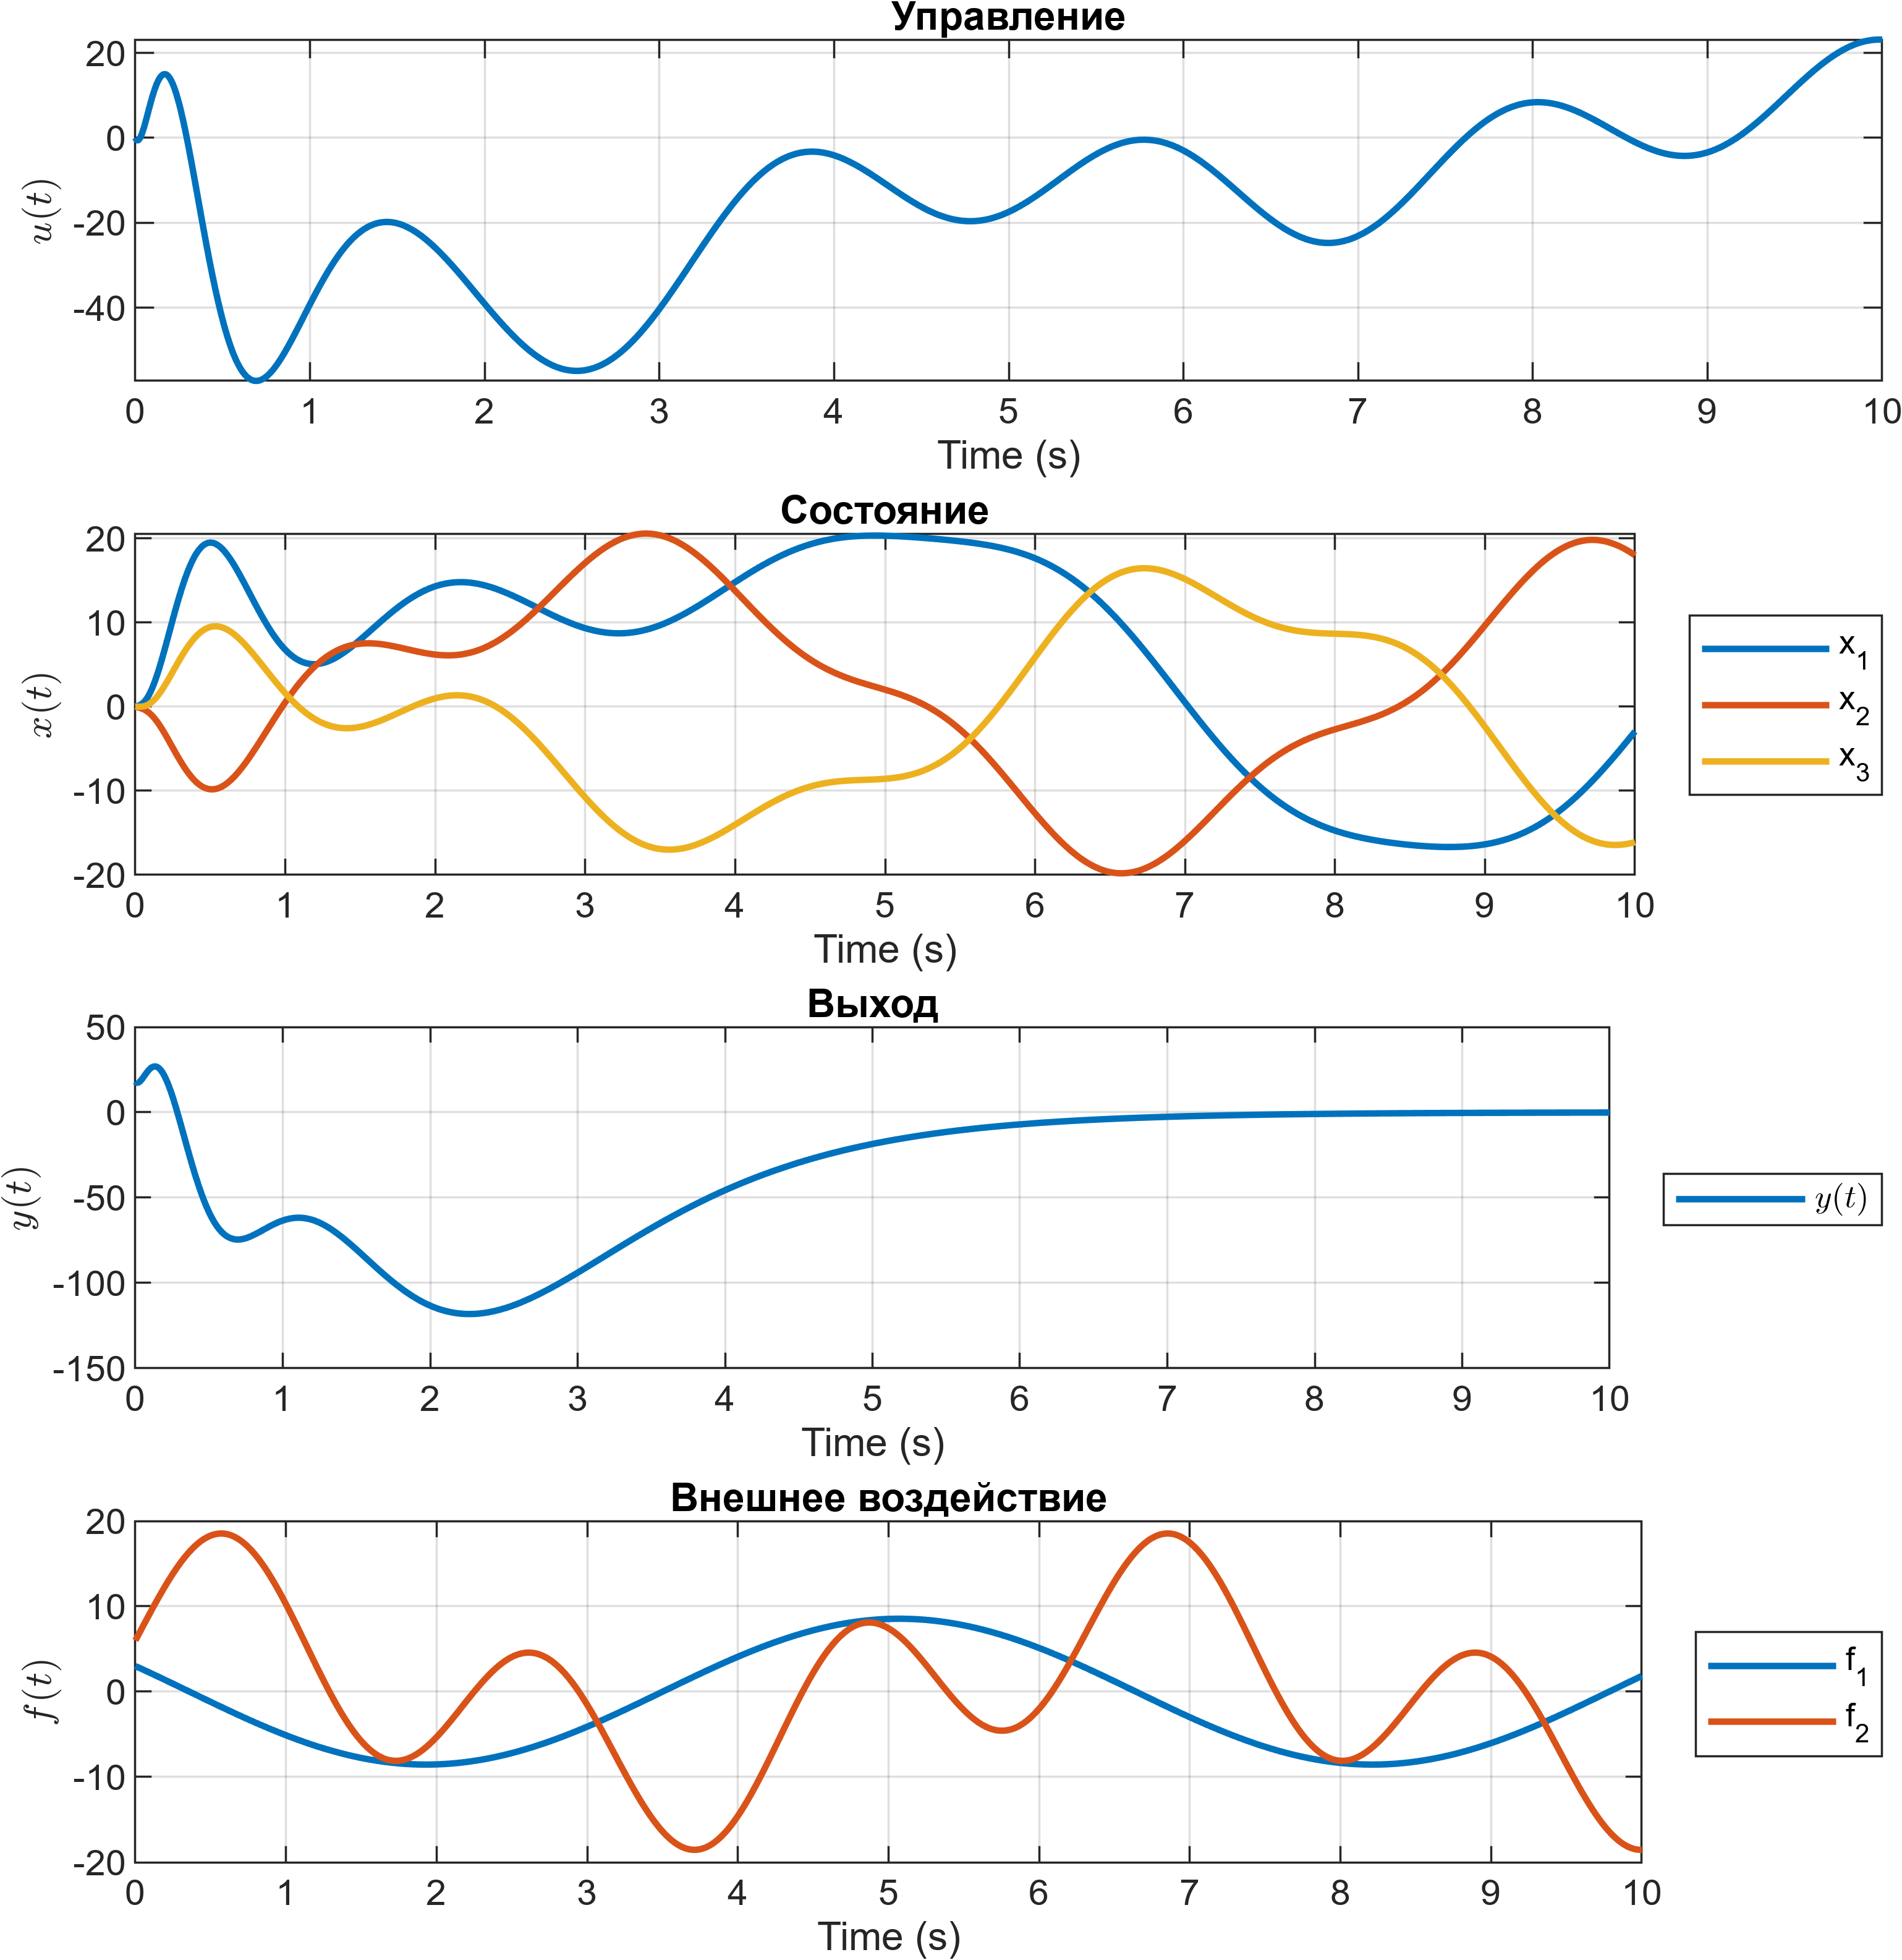
\includegraphics[width=\linewidth]{figs/2_0_sim.png}
    \caption{Графики  внешнего возмущения $f(t)$, выхода
    $y(t)$, управления $u(t)$ и вектора состояния замкнутой системы $x(t)$}
    \label{fig:2_0_sim}
\end{figure}



\subsection{С наблюдателем}

\subsubsection{Структурная схема}

Примем вектор состояния $x(t)$ недоступным к измерению. Будем использовать
уже синтезированный наблюдатель в \autoref{eq:obs}.
\begin{figure}[H]
    \centering
    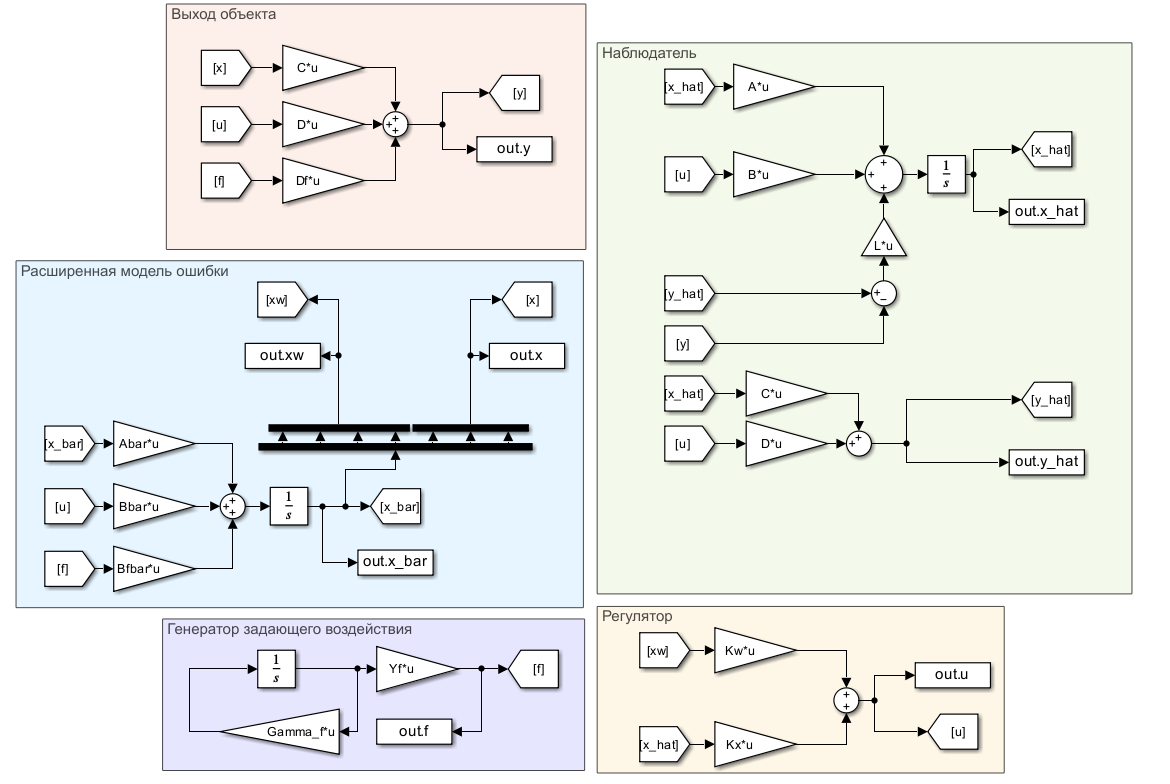
\includegraphics[width=\linewidth]{figs/2_1_slx.png}
    \caption{Структурная схема системы \eqref{eq:sys1}, замкнутой регулятором
    \eqref{eq:reg21}}
    \label{fig:21slx}
\end{figure}
\noindent Построим схему моделирования системы \eqref{eq:sys1}, замкнутой регулятором
\begin{equation}
    \label{eq:reg21}
    u=K_wx_w+K_x\hat x
\end{equation}
с наблюдателем \eqref{eq:obs1},
обеспечивающим выполнение целевого условия \eqref{eq:aim2}. Матрицы $K_w$, $K_x$
берем из $K$ \autoref{sec:reg21}:
\begin{equation*}
    K=\begin{bmatrix}
        K_w & K_x
    \end{bmatrix}.
\end{equation*}
Схему можно увидеть на \autoref{fig:21slx}. 

\subsubsection{Передаточная функция}

Определим ПФ от задающего воздействия к ошибке слежения. Для этого определим новую 
внутренную модель ошибки слежения:
\begin{equation*}
    \begin{cases}
        \dot x_w=\Gamma_fx_w+G\hat y\\
        \dot x=Ax+Bu\\
        \dot{\hat x}=A\hat x+Bu+L(\hat y - y)
    \end{cases}\Rightarrow
    \begin{cases}
        \dot x_w=\Gamma_fx_w+GC\hat x+GDu+GD_ff\\
        \dot x=Ax+Bu\\
        \dot{\hat x}=-LCx+(A+LC)\hat x+Bu
    \end{cases}
\end{equation*}
Определим новую систему
\begin{equation*}
    \dot{\tilde x}=\tilde A\tilde x+\tilde B u+\tilde B_ff,
\end{equation*}
где
\begin{equation*}
    \tilde x=\begin{bmatrix}
        x_w\\x\\ \hat x
    \end{bmatrix},\quad
    \tilde A=\begin{bmatrix}
        \Gamma&0&GC\\0&A&0\\0&-LC&A+LC
    \end{bmatrix},\quad
    \tilde B=\begin{bmatrix}
        GD\\B\\B
    \end{bmatrix},\quad
    \tilde B_f=\begin{bmatrix}
        GD_f\\0
    \end{bmatrix}.
\end{equation*}
Добавим выход:
\begin{equation*}
    \begin{cases}
        \dot{\tilde x}=\tilde A\tilde x+\tilde B u+\tilde B_ff\\
        y=\tilde{C}\tilde x+D_ff
    \end{cases},\quad
    \tilde C=\begin{bmatrix}
        DK_w&0&C+DK_x
    \end{bmatrix}.
\end{equation*}
Переопределим матрицу $K$:
\begin{equation*}
    K=\begin{bmatrix}
        K_w&0&K_x
    \end{bmatrix}
\end{equation*}
Проверим закнутую систему:
\begin{equation*}
    \sigma(\tilde A+\tilde BK)=\left(\begin{array}{c}
-6.0\\
-1.0\\
-5.017\\
-5.0\\
-3.968\\
-4.0\\
-3.02\\
-3.0\\
-1.995\\
-2.0
\end{array}\right),
\end{equation*}
замкнутая система устойчива и содержит спектр наблюдателя, замкнутой системы и одно неуправляемое
собственное число.
Формула ПФ:
\begin{equation*}
    \underset{f\rightarrow y}{W}=\tilde C(sI-(\tilde A+\tilde BK))^{-1}\tilde B_f+D_f,
\end{equation*}
с помощью MATLAB получим
\begin{equation*}
    \underset{f\rightarrow y}{W} =
    \left(\begin{array}{cc}
        \frac{256.0\,\sigma_2}{\sigma_1} & \frac{64.0\,\sigma_2}{\sigma_1}
    \end{array}\right)
    \begin{array}{l}
        \sigma_1 = 6.669 \cdot 10^{57}s^9 + 1.679 \cdot 10^{59}s^8 - 9.532 \cdot 10^{59}s^7 - 1.471 \cdot 10^{61}s^6 -\\
        \quad 1.545 \cdot 10^{61}s^5 + 1.199 \cdot 10^{62}s^4 + 2.038 \cdot 10^{62}s^3 + 4.727 \cdot 10^{62}s^2 +\\
        \quad 1.111 \cdot 10^{63}s - 1.217 \cdot 10^{63},\\[8pt]
        \sigma_2 = 1.042 \cdot 10^{56}s^9 - 2.875 \cdot 10^{57}s^8 - 3.051 \cdot 10^{58}s^7 - 5.974 \cdot 10^{58}s^6 +\\
        \quad 5.143 \cdot 10^{58}s^5 + 4.475 \cdot 10^{59}s^4 + 3.376 \cdot 10^{60}s^3 + 7.554 \cdot 10^{60}s^2 +\\
        \quad 3.294 \cdot 10^{60}s + 7.05 \cdot 10^{60}.
    \end{array}
\end{equation*}
Данная ПФ представляет собой матрицу 1х2, так как $f$ - двумерный вектор, 
первая ПФ имеет нули $\left(\begin{array}{c}
-3.0\\
-4.0\\
-5.0\\
-6.383+15.75\,\mathrm{i}\\
-6.383-15.75\,\mathrm{i}\\
-1.0\,\mathrm{i}\\
1.0\,\mathrm{i}\\
3.0\,\mathrm{i}\\
-3.0\,\mathrm{i}
\end{array}\right)$ и полюса $\left(\begin{array}{c}
-1.0\\
-1.995\\
-3.0\\
-3.02\\
-3.968\\
-4.0\\
-5.0\\
-5.017\\
-6.0
\end{array}\right)$,
вторая ПФ имеет нули $\left(\begin{array}{c}
-3.0\\
-4.0\\
-5.0\\
-6.383+15.75\,\mathrm{i}\\
-6.383-15.75\,\mathrm{i}\\
-1.0\,\mathrm{i}\\
1.0\,\mathrm{i}\\
3.0\,\mathrm{i}\\
-3.0\,\mathrm{i}
\end{array}\right)$ и полюса $\left(\begin{array}{c}
-1.0\\
-1.995\\
-3.0\\
-3.02\\
-3.968\\
-4.0\\
-5.0\\
-5.017\\
-6.0
\end{array}\right)$,
как видно, нули содержат спектр задающего воздействия, что 
соответствует принципу внутренней модели, которым мы руководствовались, этот же спектр 
содержит нули ПФ для случая без наблюдателя и 
дополнительно спектр наблюдателя ($A+LC$); полюса так же содержат полюса ПФ случая без
наблюдателя и дополнительно спектр наблюдателя ($A+LC$).
Проверим выполнение целевого условия \eqref{eq:aim2}, используя теорему о предельном
значении:
\begin{multline*}
    \lim_{t\rightarrow\infty}|y(t)|=\lim_{s\rightarrow0}|sY(s)|=
    \lim_{s\rightarrow0}|s\underset{f\rightarrow y}{W}(s)F(s)|=
    \lim_{s\rightarrow0}|s\underset{f\rightarrow y}{W}(s)(Y_f(sI-\Gamma_f)^{-1}w_{f}(0))|=\\
    \lim_{s\rightarrow0}\Bigg|s\frac{64.0\,\Big(1.876 \cdot 10^{57}s^{12} - 5.165 \cdot 10^{58}s^{11} + \dots - 1.628 \cdot 10^{63}\Big)}{
    6.669 \cdot 10^{57}s^{13} + 1.679 \cdot 10^{59}s^{12} + \dots - 1.096 \cdot 10^{64}}\Bigg|=0.
\end{multline*}
Условие выполняется.

\subsubsection{Моделирование}

Выполним компьютерное моделирование системы, замкнутой регулятором
\eqref{eq:reg21} и наблюдателем \eqref{eq:obs1} с единичными начальными условиями, 
и построим графики формируемого 
регулятором управления $u(t)$, вектора состояния замкнутой системы $x(t)$, его оценки и их разности, выхода
$y(t)$. Графики можно
увидеть на рисунках \ref{fig:2_1_0_sim} и \ref{fig:2_1_1_sim}.

\begin{figure}[H]
    \centering
    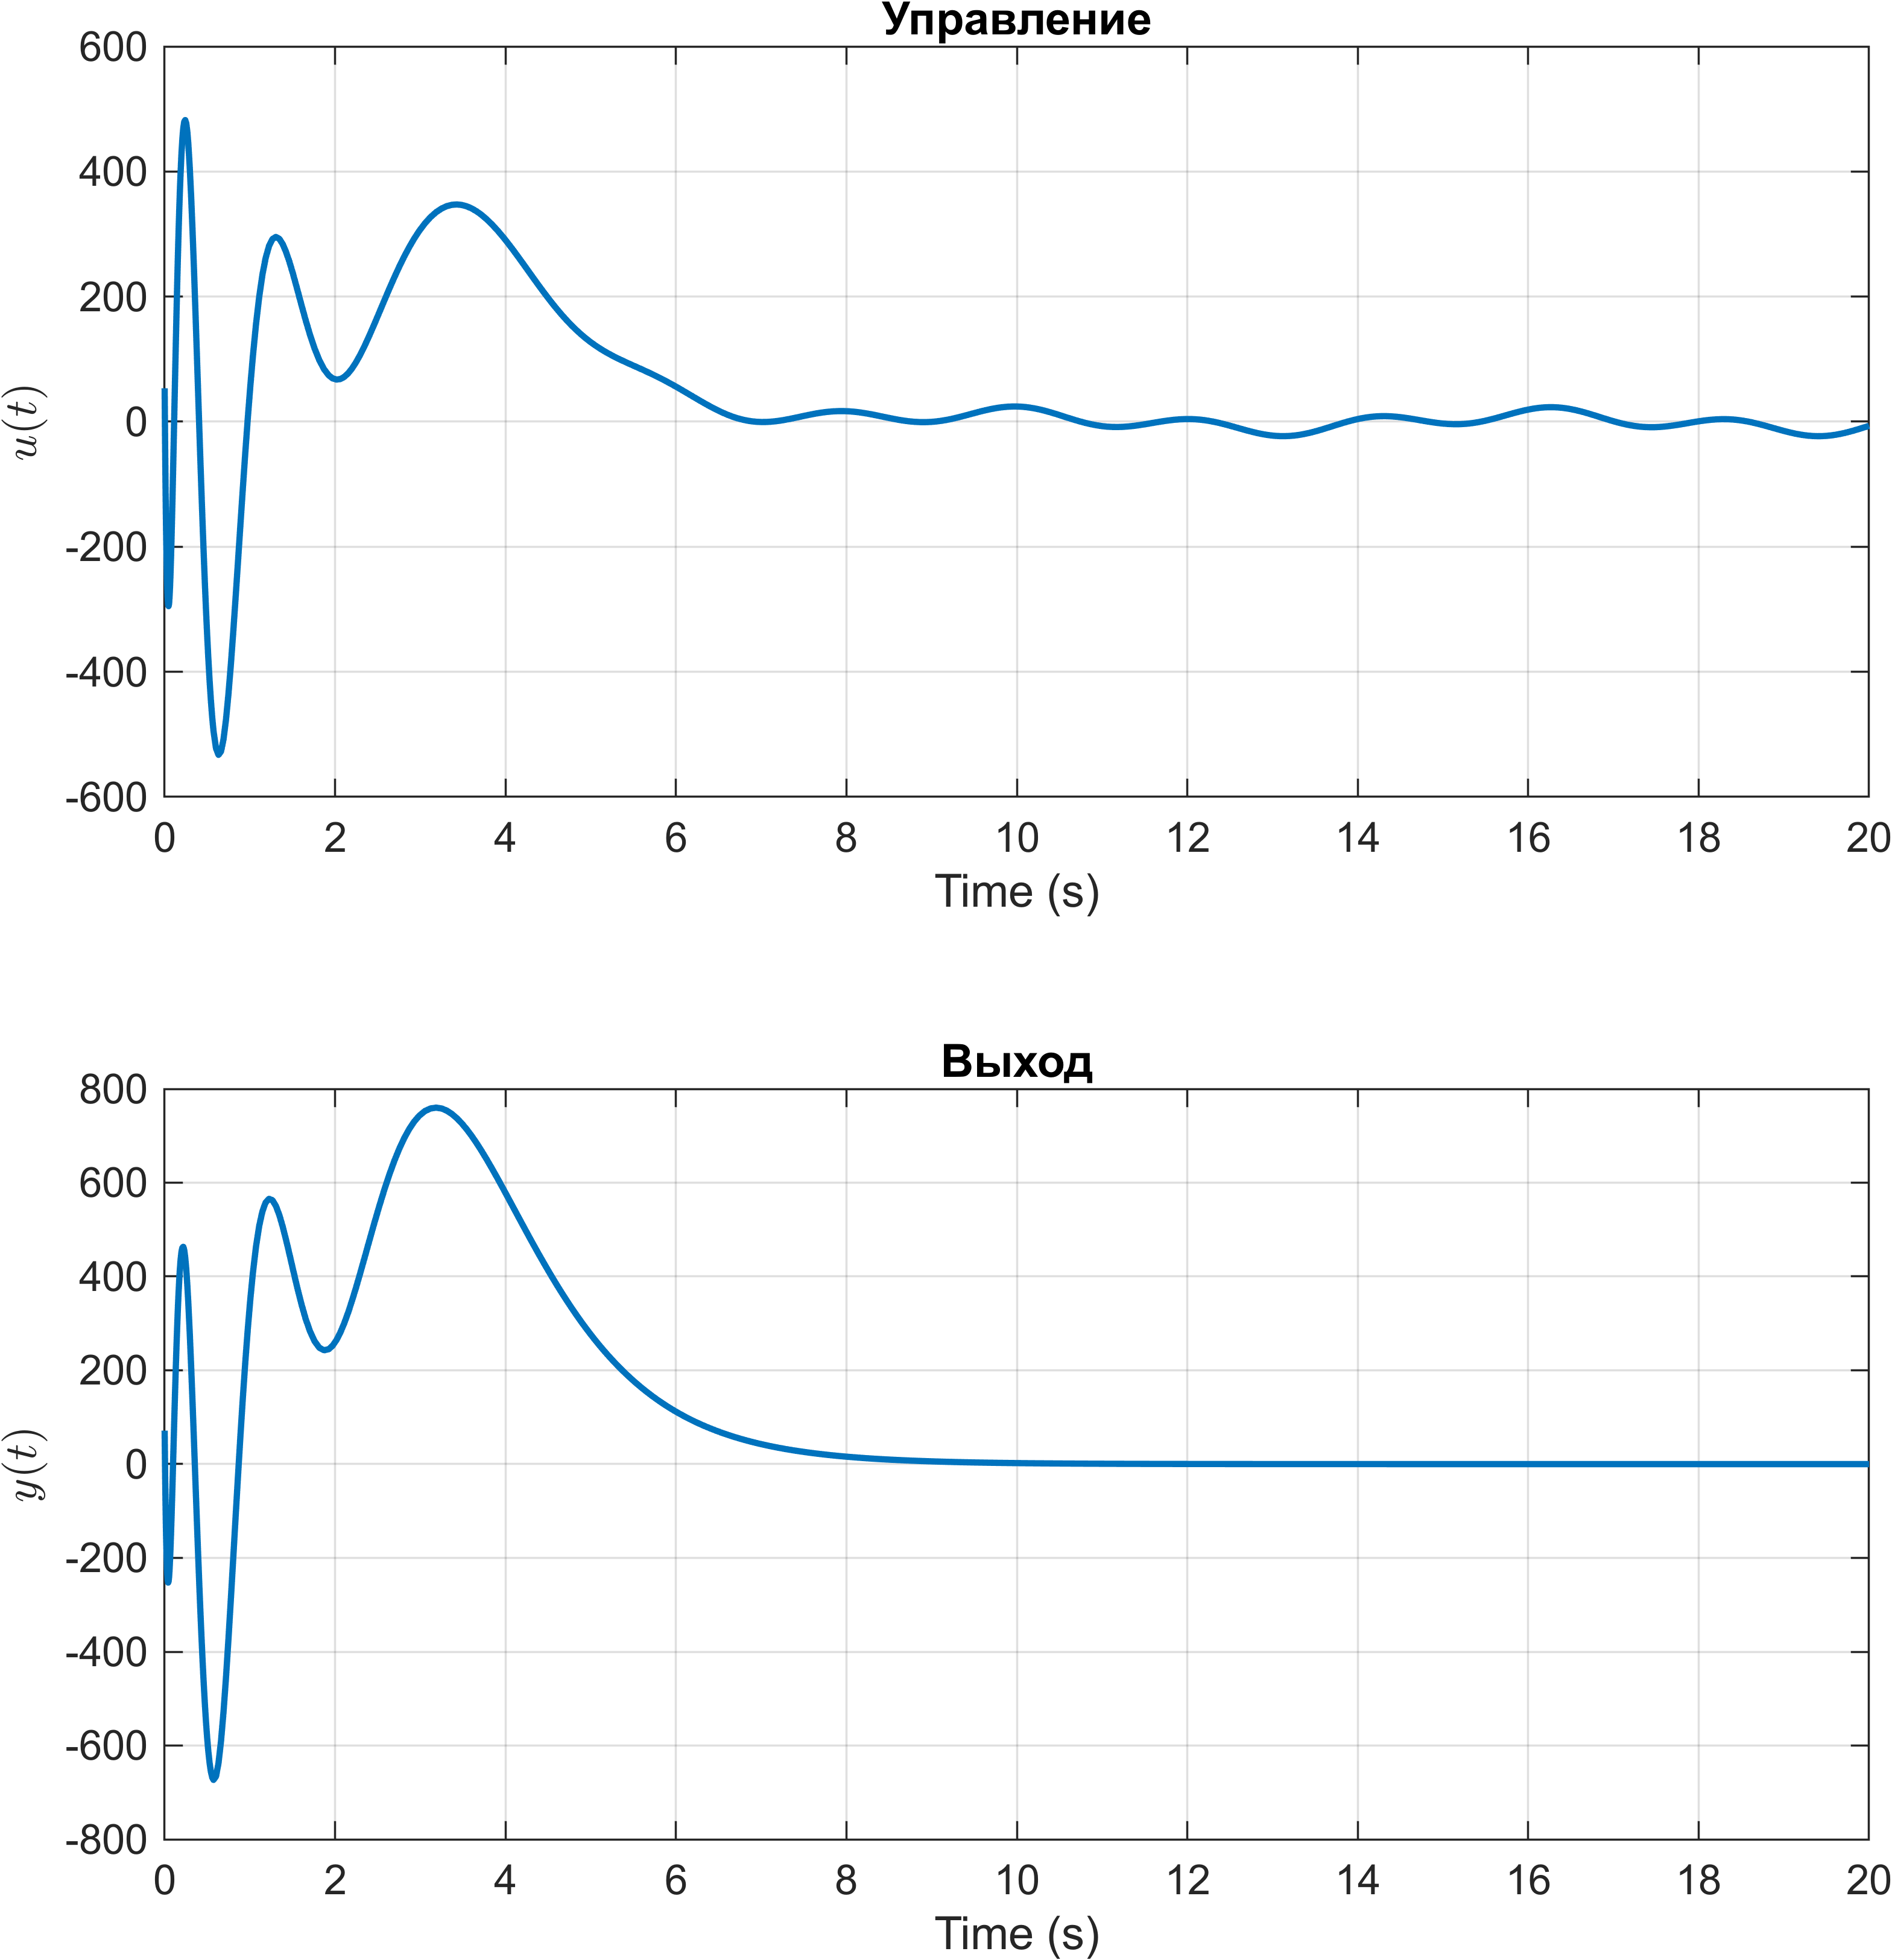
\includegraphics[width=\linewidth]{figs/2_1_0_sim.png}
    \caption{Графики выхода
    $y(t)$ и управления $u(t)$}
    \label{fig:2_1_0_sim}
\end{figure}

\begin{figure}[H]
    \centering
    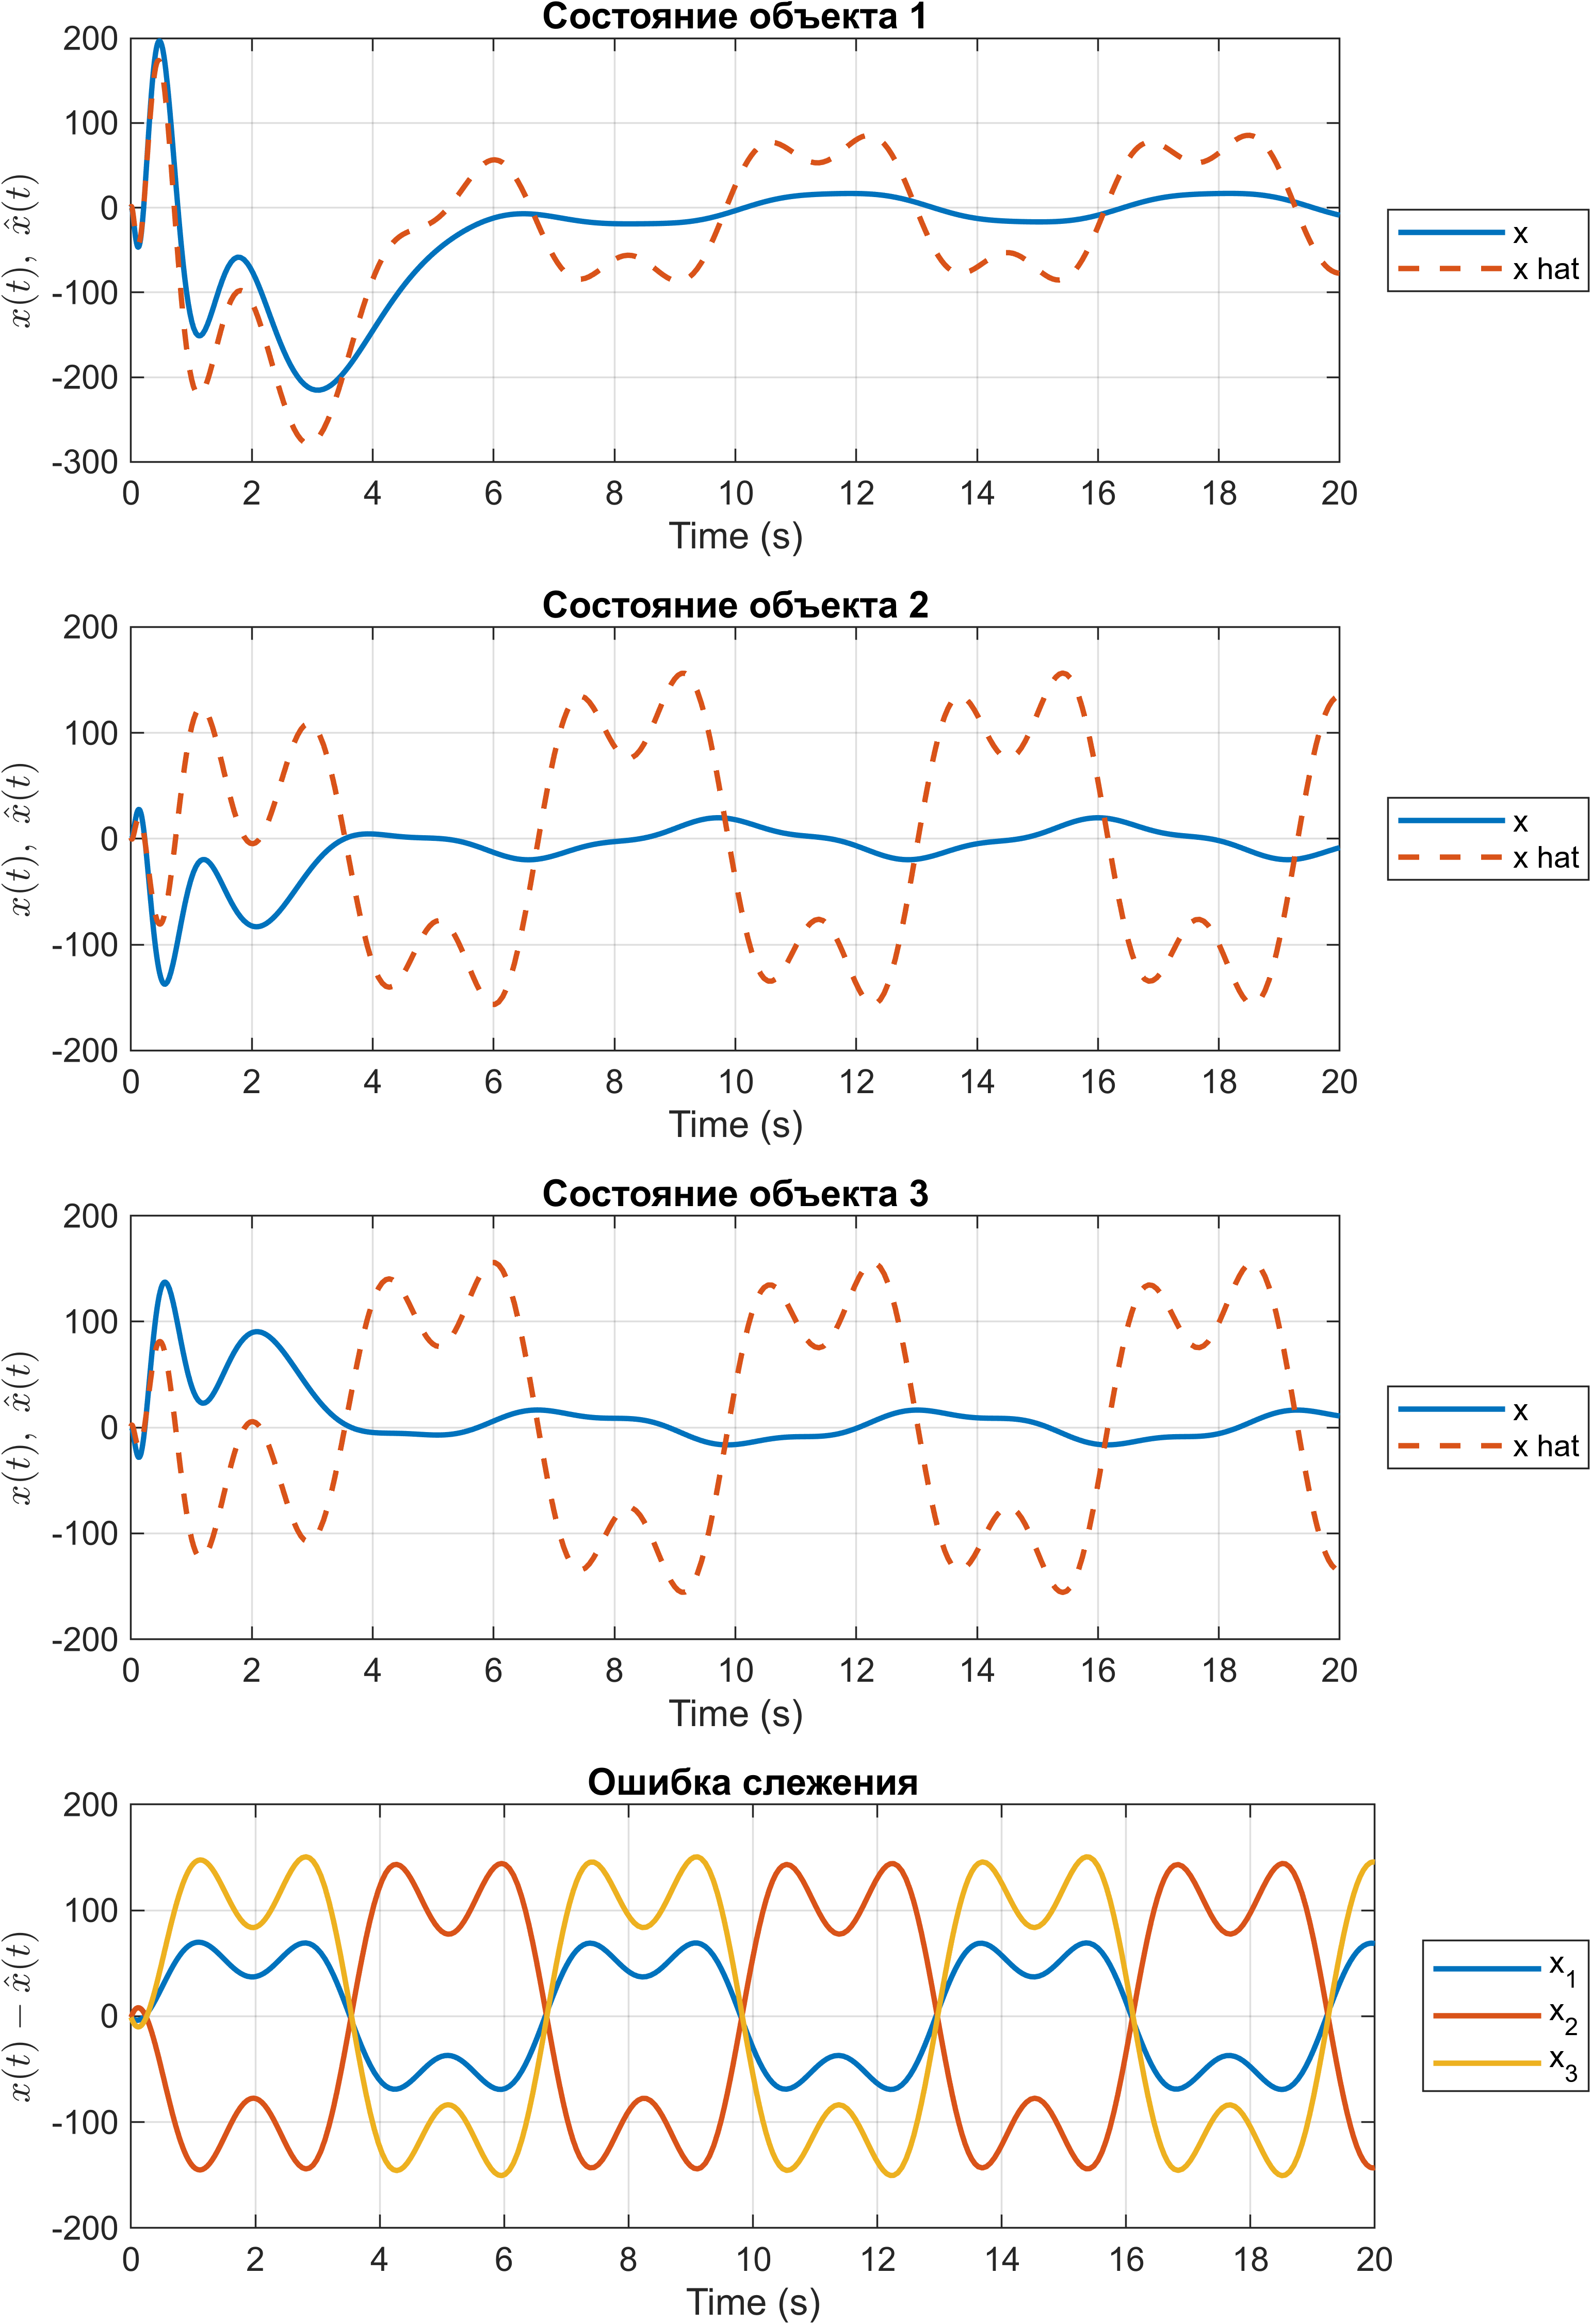
\includegraphics[width=\linewidth]{figs/2_1_1_sim.png}
    \caption{Графики вектора состояния замкнутой системы $x(t)$, его оценки наблюдателем и 
    их разности}
    \label{fig:2_1_1_sim}
\end{figure}


\subsection{Выводы}

Была рассмотрена компенсация с помощью режекторной фильтрации с и без наблюдателя состояния.
В обоих случаях выполняется принцип внутренней модели. Моделирование показало,
что в обоих случаях система успешно компенсировала внешнее возмущение. Отмечу, что система с наблюдателем
успешно справилась с задачей, на 20 секунде моделирования значение $y$ составило 9.83e-05, несмотря на то что
наблюдатель не имел понятия о внешнем воздействии, что отразилось на постоянно колеблющейся ошибке
оценки состояния.



\section{Режекторная фильтрация: Все разом}

\subsection{Анализ системы}

Рассмотрим систему \eqref{eq:sys1}:
\begin{equation}
    \begin{cases}
        \dot x = Ax+Bu+B_ff,\\
        y=Cx+Du+D_ff,
    \end{cases}\quad x(0)=\begin{bmatrix}
        0&0&0
    \end{bmatrix}^T,
\end{equation}
где
\begin{equation*}
    A=\begin{bmatrix}
        3 & 5 & 4 \\
        -2 & -4 & -5 \\
        2 & 2 & 3
    \end{bmatrix},\quad
    B=\begin{bmatrix}
        2 \\ -1 \\ 1
    \end{bmatrix},\quad
    B_f=\begin{bmatrix}
        -2 & 2 \\ -2 & 0 \\ 0 & 0
    \end{bmatrix},
\end{equation*}
\begin{equation*}
    C=\begin{bmatrix}
        -2&-1&0
    \end{bmatrix},\quad
    D=\begin{bmatrix}
        1
    \end{bmatrix},\quad
    D_f=\begin{bmatrix}
        4&1
    \end{bmatrix},
\end{equation*}
генератор внешнего воздействия
\begin{equation}
    \label{eq:sys_fg}
    \begin{cases}
        \dot w=\Gamma_ww,\\
        g=\bar Y_gw_w,\\
        f=\bar Y_fw_w,
    \end{cases},\quad     w_w(0)=\begin{bmatrix}
        1&1&1&1&1&0&1
    \end{bmatrix}^T,
\end{equation}
где
\begin{equation*}
    \Gamma_w=\begin{bmatrix}
        35& 56& 22& -42 & 0 & 0 & 0\\
        -11& -17& -7& 12 & 0 & 0 & 0\\
        -6& -10& -5& 10 & 0 & 0 & 0\\
        11 &18& 6& -13 & 0 & 0 & 0\\
        0 & 0 & 0 & 0 & 0 & 5 & 0 \\
        0 & 0 & 0 & 0 & -5& 0 & 0 \\
        0 & 0 & 0 & 0 & 0 & 0 & 0
    \end{bmatrix},\quad
    \bar Y_g=\begin{bmatrix}
        0\\0\\0\\0\\8 \\ 0 \\ 2
    \end{bmatrix}^T,\quad
    \bar Y_f=\begin{bmatrix}
        1&3\\2&4\\1&2\\-1&-3\\0&0\\0&0\\0&0\\
    \end{bmatrix}^T.
\end{equation*}
Внутренняя модель:
\begin{equation*}   
    \begin{cases}
        \dot e_w=\Gamma_w e_w+G\varepsilon,\\
        \varepsilon=g-y.
    \end{cases}
\end{equation*}
Зададимся матрицей $G$ исходя из условия управляемости пары $(\Gamma_w,\ G)$:
\begin{equation*}
    G=\begin{bmatrix}
        1&1&1&1&1&1&1
    \end{bmatrix}^T.
\end{equation*}
Определим матрицы расширенной модели ошибки
\begin{equation*}
    \dot{\bar e}=\bar A\bar e+\bar Bu+\bar Gg+\bar B_ff,
\end{equation*}
где
\begin{equation*}
    \bar e=\begin{bmatrix}
        e_w\\x
    \end{bmatrix},\quad
    \bar A=\begin{bmatrix}
        \Gamma_w&-GC\\0&A
    \end{bmatrix},\quad
    \bar B=\begin{bmatrix}
        -GD\\B
    \end{bmatrix},\quad
    \bar G=\begin{bmatrix}
        G\\0
    \end{bmatrix},\quad
    \bar B_f=\begin{bmatrix}
        -GD_f\\B_f
    \end{bmatrix}.
\end{equation*}



\subsection{Без наблюдателя}

\begin{figure}[H]
    \centering
    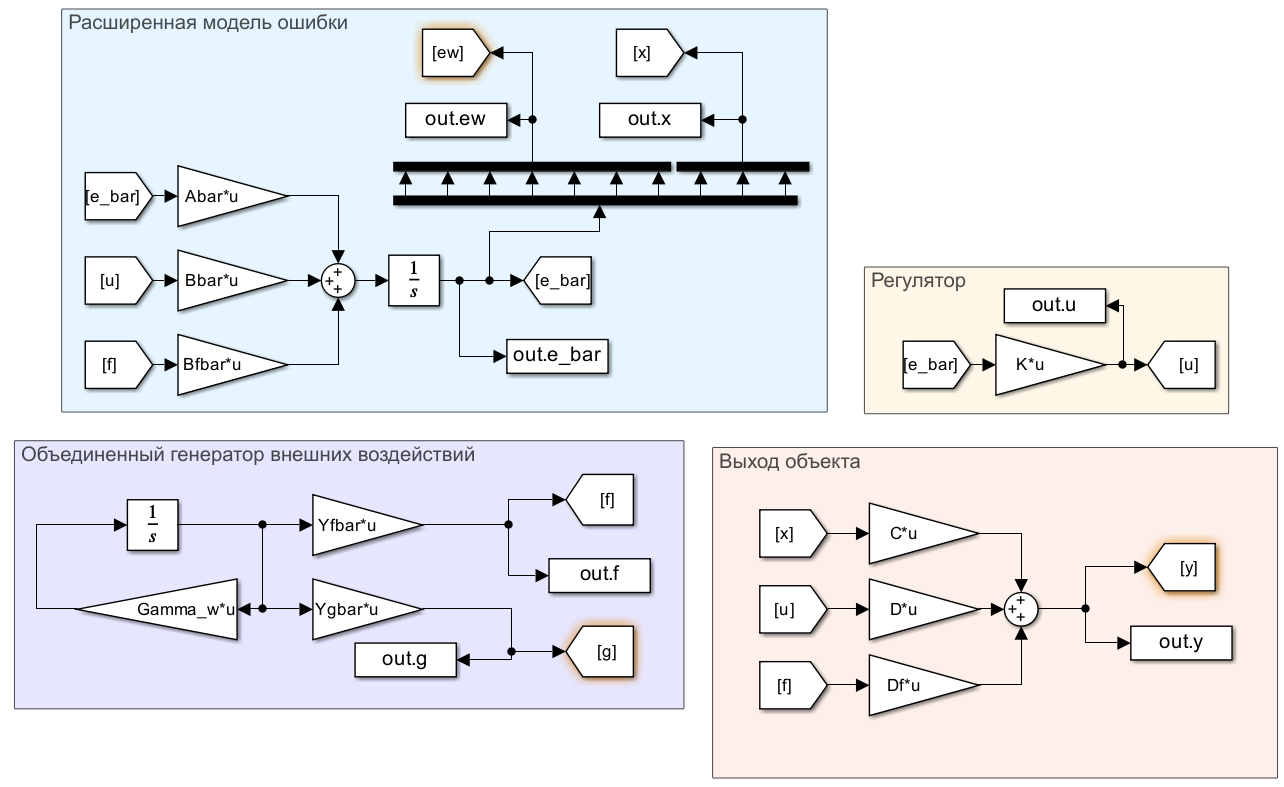
\includegraphics[width=\linewidth]{figs/3_0_slx.png}
    \caption{Структурная схема системы \eqref{eq:sys1}, замкнутой регулятором
    \eqref{eq:reg3}}
    \label{fig:30slx}
\end{figure}

Примем вектор состояния системы $x(t)$ доступным к измерению.
Построим схему моделирования системы \eqref{eq:sys1}, замкнутой регулятором
\begin{equation}
    \label{eq:reg3}
    u=K\bar e,
\end{equation}
обеспечивающим выполнение целевого условия \eqref{eq:aim}. Схему можно увидеть на 
\autoref{fig:30slx}.
Аналогично предыдущим случаям выберем матрицы $\Gamma$ и $Y$ для синтеза регулятора
\begin{equation*}
    \Gamma=\begin{bmatrix}
        -1 & 0 & 0 & 0 & 0 & 0 & 0 & 0 & 0\\
        0 & -3 & 0 & 0 & 0 & 0 & 0 & 0 & 0\\
        0 & 0 & -4 & 0 & 0 & 0 & 0 & 0 & 0\\
        0 & 0 & 0 & -5 & 0 & 0 & 0 & 0 & 0\\
        0 & 0 & 0 & 0 & -6 & 0 & 0 & 0 & 0\\
        0 & 0 & 0 & 0 & 0 & -7 & 0 & 0 & 0\\
        0 & 0 & 0 & 0 & 0 & 0 & -8 & 0 & 0\\
        0 & 0 & 0 & 0 & 0 & 0 & 0 & -9 & 0\\
        0 & 0 & 0 & 0 & 0 & 0 & 0 & 0 & -10
    \end{bmatrix},\quad
    Y=\begin{bmatrix}
        1 \\ 1 \\ 1 \\ 1 \\ 1 \\ 1 \\ 1 \\ 1 \\ 1
    \end{bmatrix}^T,
\end{equation*}
и получим 
\begin{equation*}
    K=\begin{bmatrix}
        890.1 & 1378.0 & 626.5 & -1118.0 & 189.2 & 41.64 & 672.0 & 4359.0 & 3047.0 & -3047.0
    \end{bmatrix}.
\end{equation*}
Выполним компьютерное моделирование системы, замкнутой регулятором
\eqref{eq:reg3} и построим графики задающего воздействия $g(t)$, возмущения $f(t)$ 
формируемого регулятором управления $u(t)$, вектора состояния замкнутой 
системы $x(t)$, выхода $y(t)$ и ошибки регулирования $\varepsilon(t) = g(t) - y(t)$.
Графики можно увидеть на \autoref{fig:3_0_sim}.

\begin{figure}[H]
    \centering
    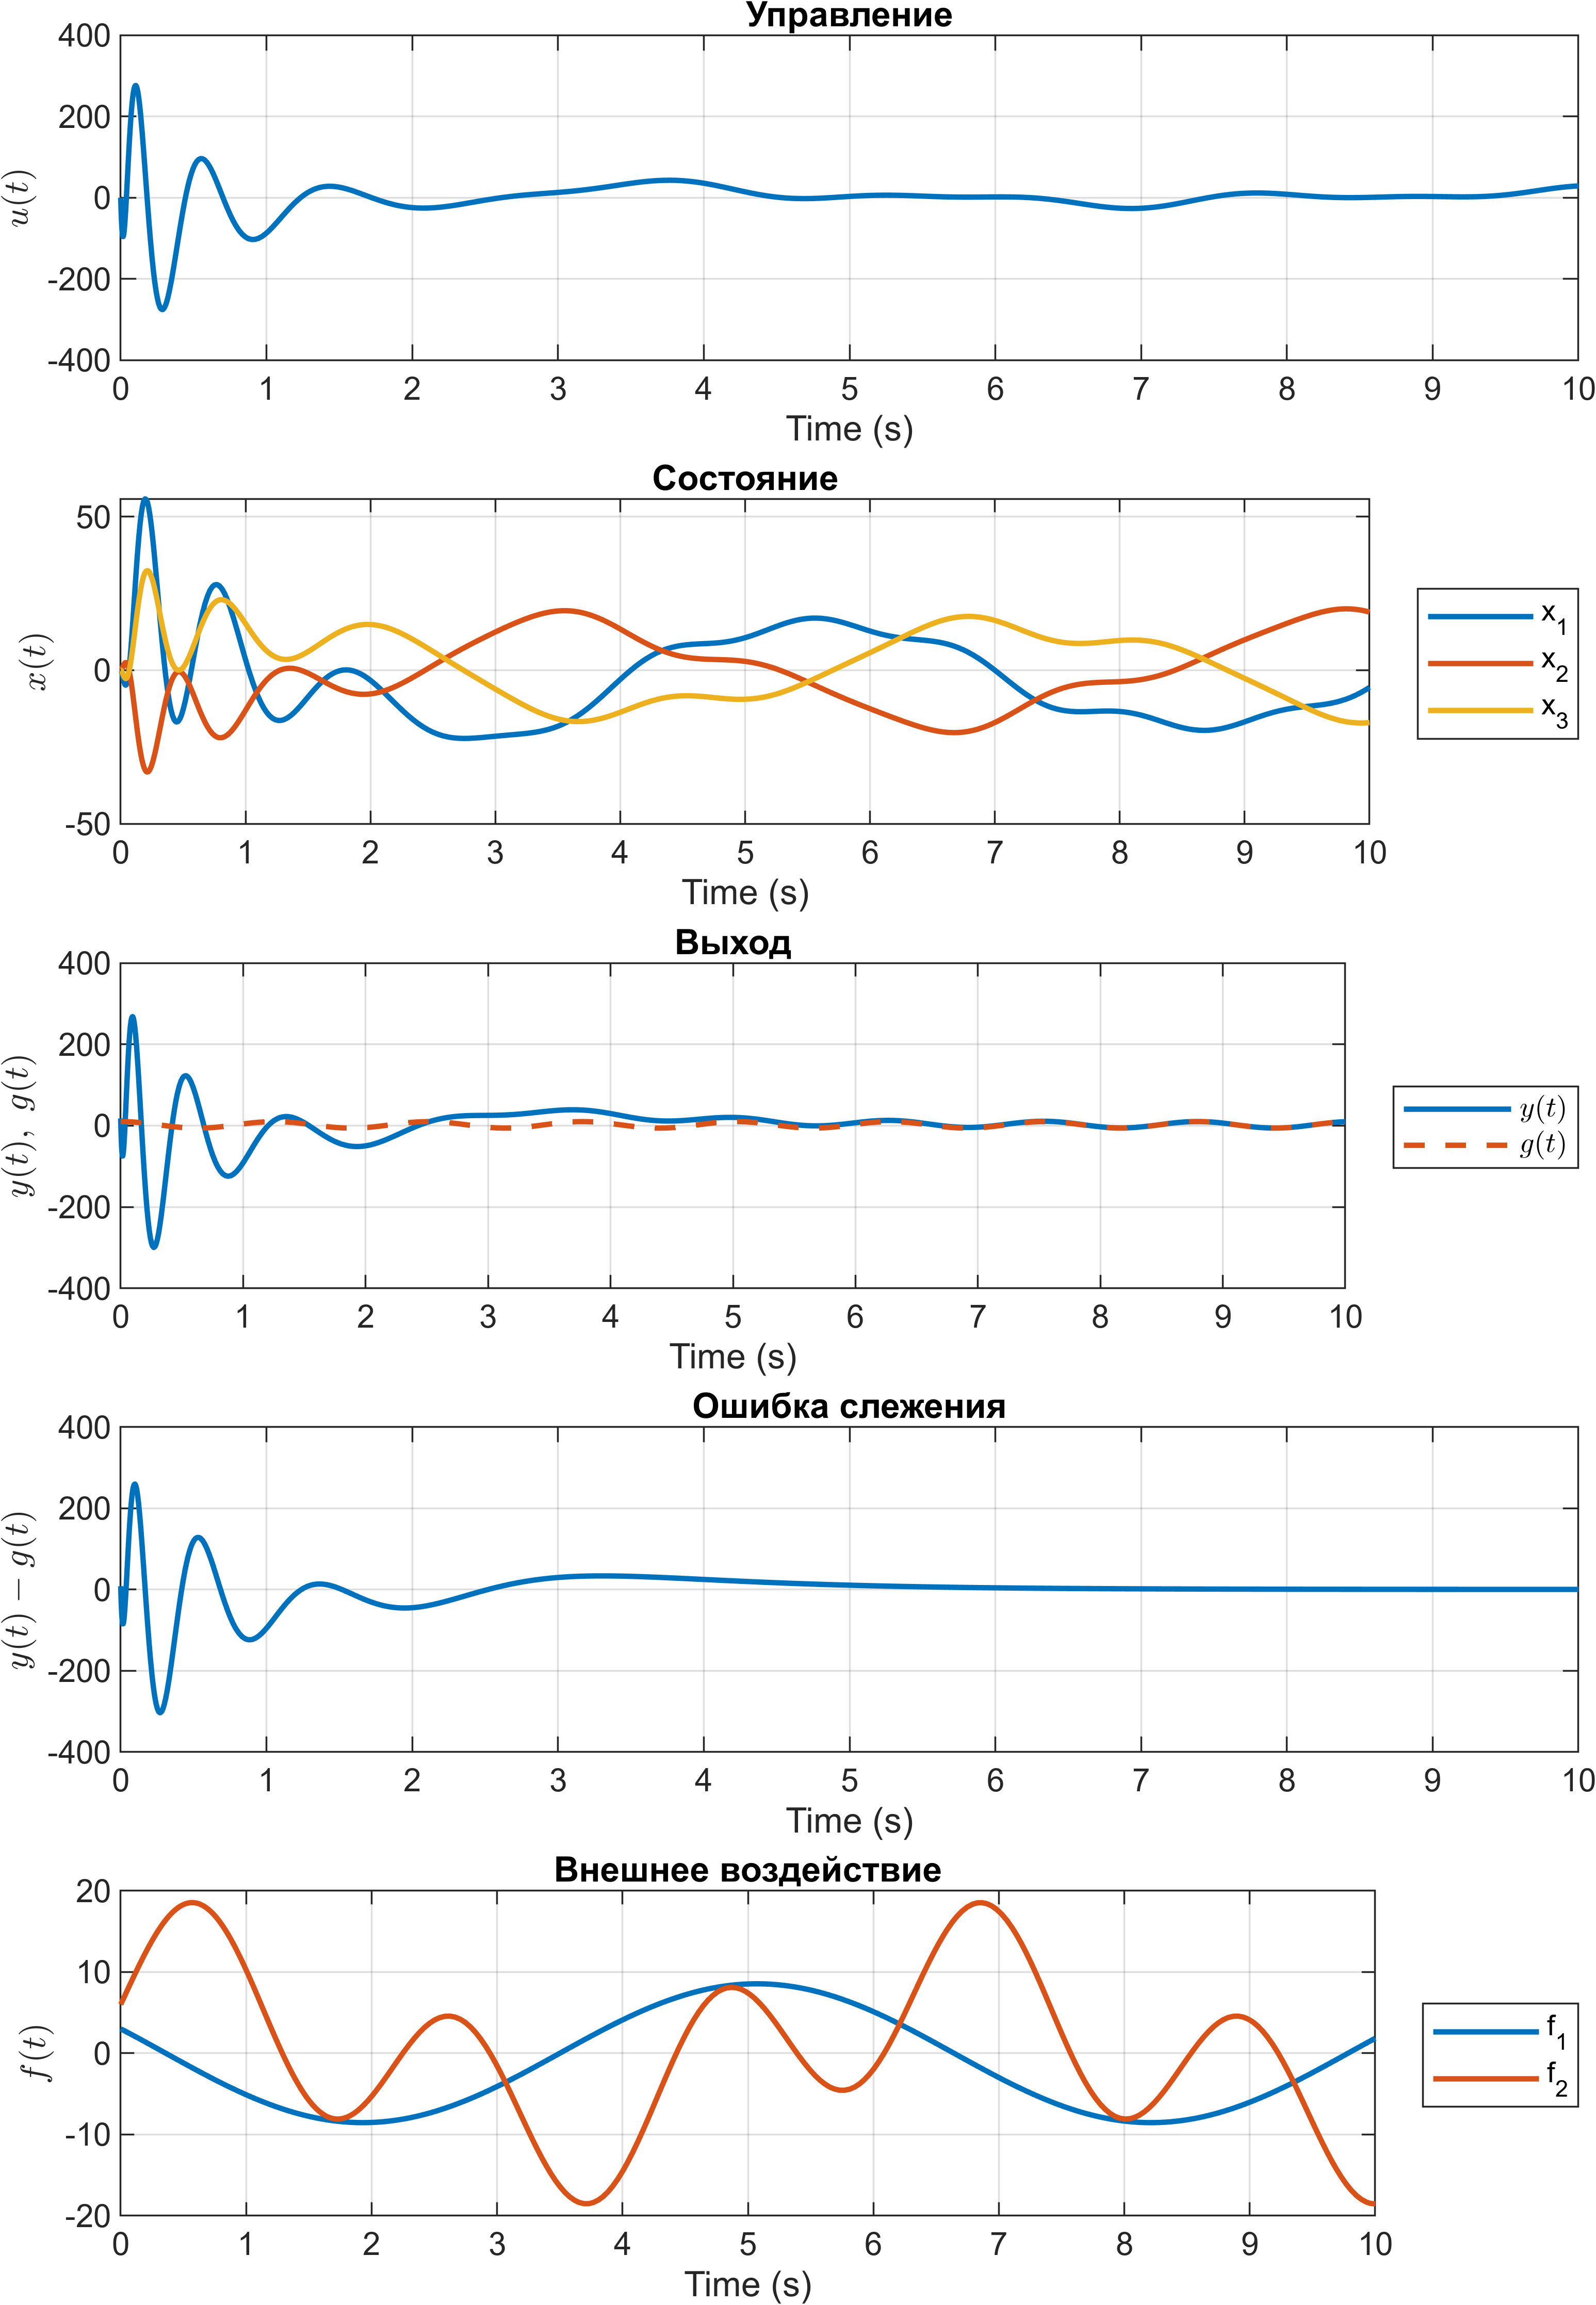
\includegraphics[width=\linewidth]{figs/3_0_sim.png}
    \caption{Графики  внешнего возмущения $f(t)$, выхода
    $y(t)$, управления $u(t)$ и вектора состояния замкнутой системы $x(t)$,
    а так же задающего воздействия $g(t)$ и ошибки регулирования $\varepsilon(t) = g(t) - y(t)$}
    \label{fig:3_0_sim}
\end{figure}


\subsection{С наблюдателем}

\begin{figure}[H]
    \centering
    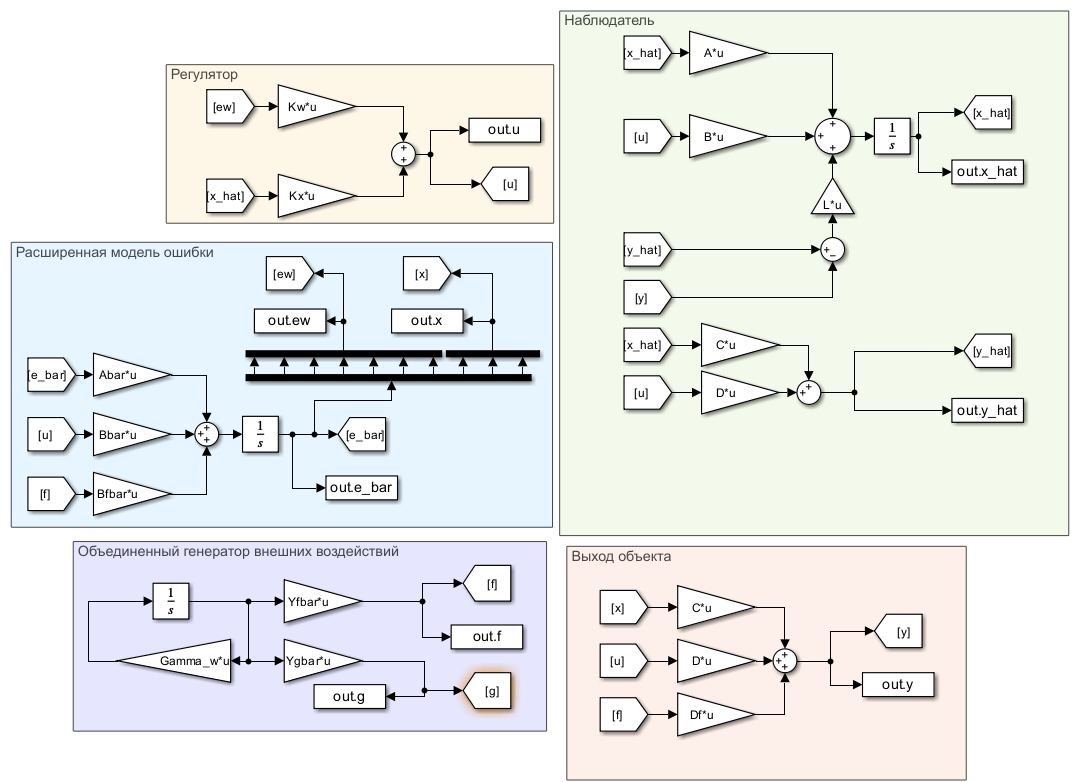
\includegraphics[width=\linewidth]{figs/3_1_slx.png}
    \caption{Структурная схема системы \eqref{eq:sys1}, замкнутой регулятором
    \eqref{eq:reg3} с наблюдателем \eqref{eq:obs1}}
    \label{fig:31slx}
\end{figure}

Примем вектор состояния системы $x(t)$ недоступным к измерению.
Построим схему моделирования системы \eqref{eq:sys1}, замкнутой регулятором
\eqref{eq:reg3}, но с оценкой состояния от наблюдателя \eqref{eq:obs1},
обеспечивающим выполнение целевого условия \eqref{eq:aim}. Схему можно увидеть на 
\autoref{fig:31slx}.
Выполним компьютерное моделирование системы, замкнутой регулятором
\eqref{eq:reg3} с заменой вектора состояния $x(t)$ на его оценку $\hat x(t)$, 
и постром графики
формируемого регулятором управления $u(t)$, вектора состояния замкнутой
системы $x(t)$, его оценки $\hat x(t)$, невязки $e_x(t) = x(t)-\hat x(t)$, 
выхода $y(t)$ и ошибки регулирования $\varepsilon(t) = g(t) - y(t)$.
Графики можно увидеть на \autoref{fig:3_0_sim}.

\begin{figure}[H]
    \centering
    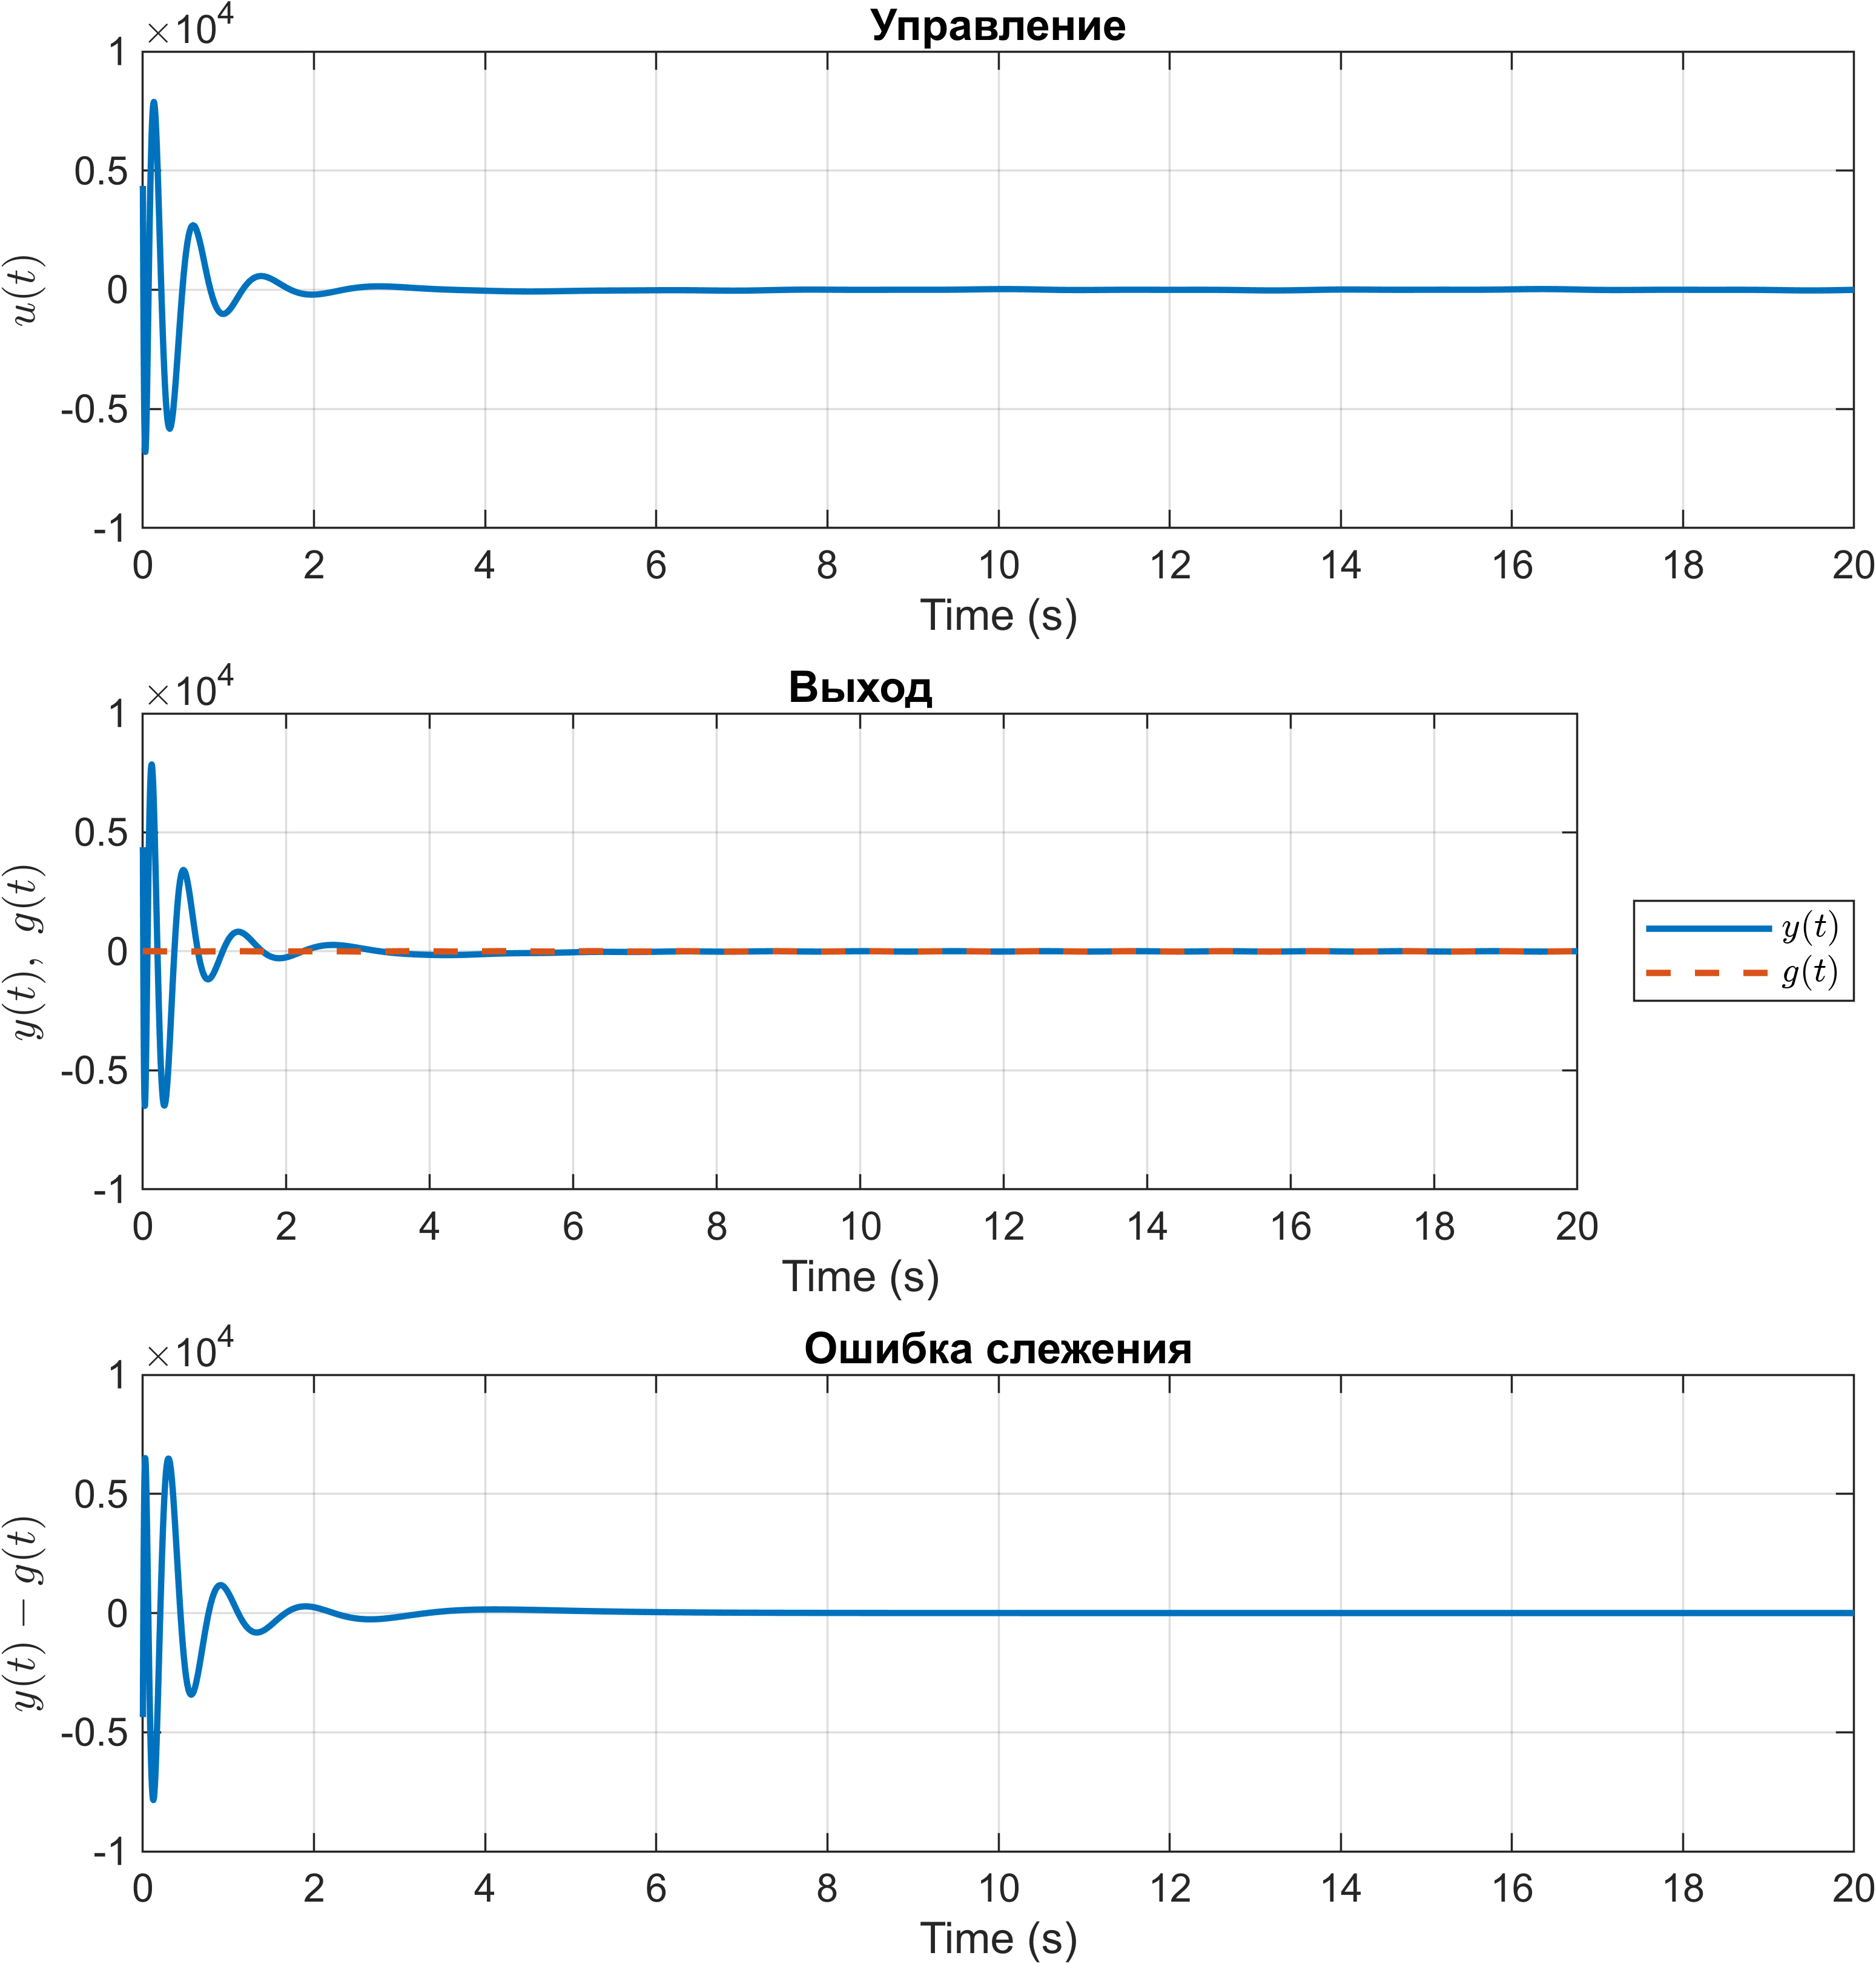
\includegraphics[width=\linewidth]{figs/3_1_0_sim.png}
    \caption{Графики выхода $y(t)$, управления $u(t)$
    и ошибки регулирования $\varepsilon(t) = g(t) - y(t)$}
    \label{fig:3_1_0_sim}
\end{figure}

\begin{figure}[H]
    \centering
    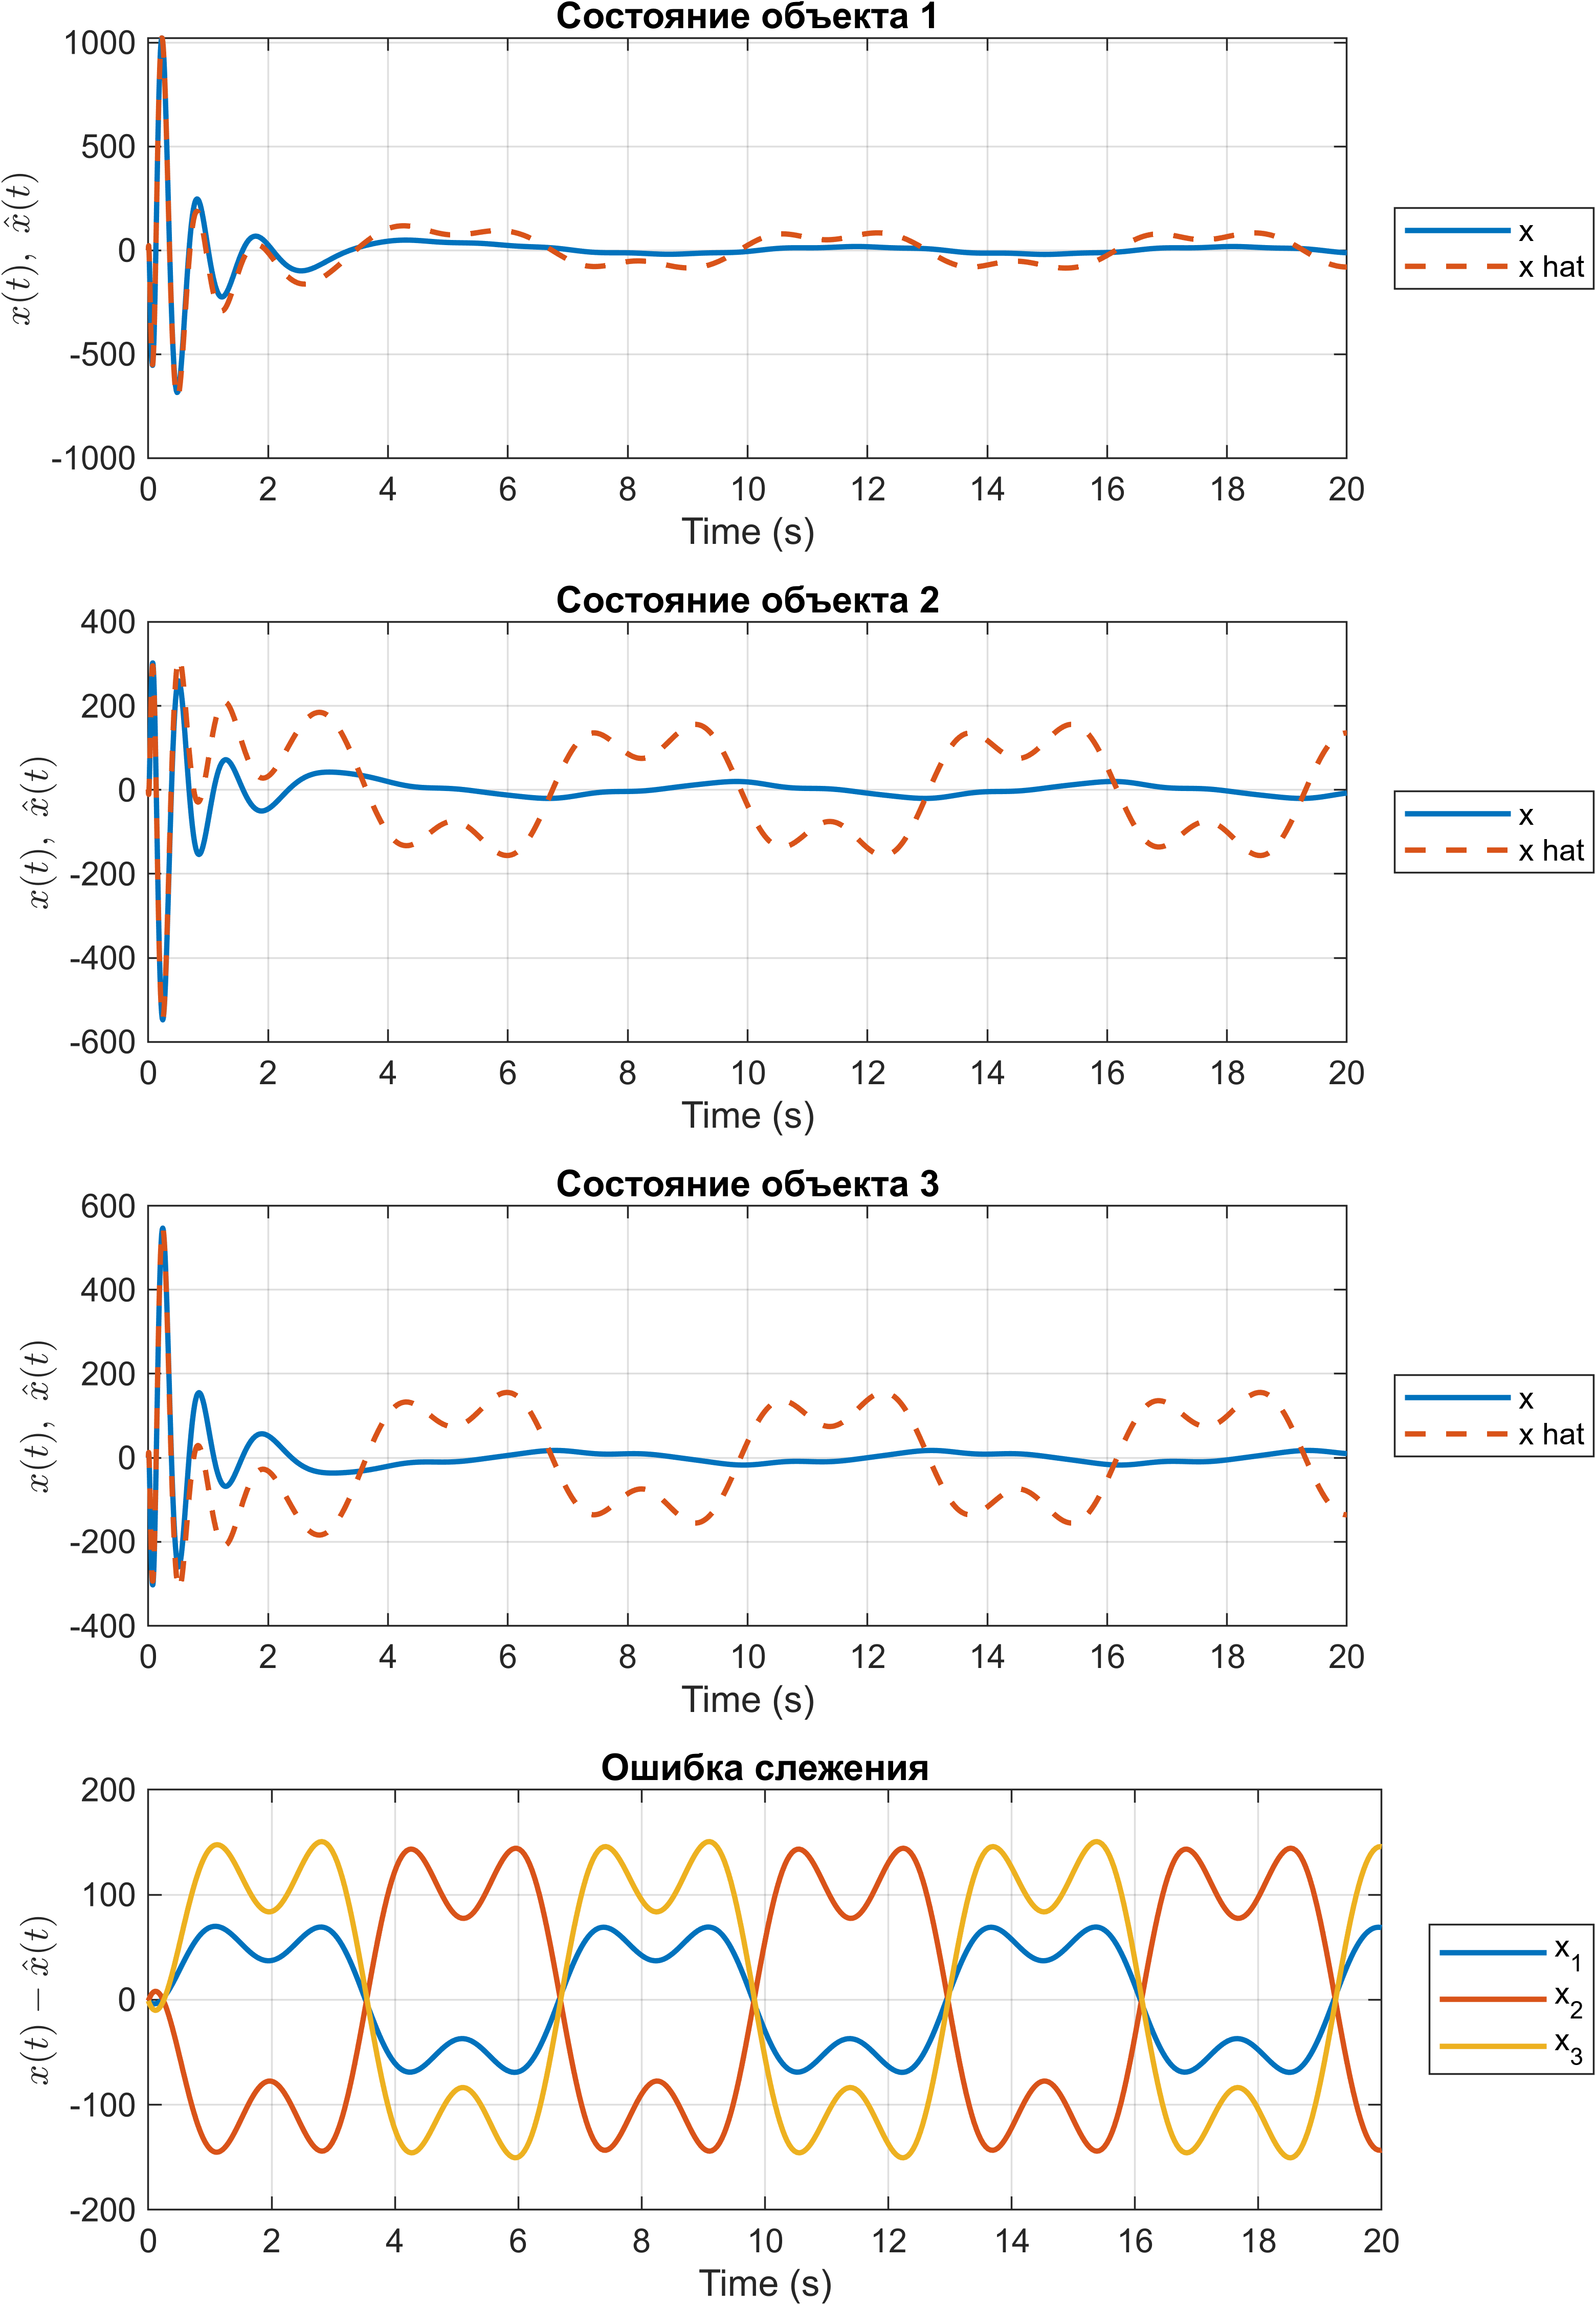
\includegraphics[width=\linewidth]{figs/3_1_1_sim.png}
    \caption{Графики вектора состояния замкнутой системы $x(t)$, 
    его оценки наблюдателем и их разности}
    \label{fig:3_1_1_sim}
\end{figure}


\subsection{Выводы}

Была рассмотрена одновременная компенсация и слежение с помощью режекторной фильтрации с и без наблюдателя состояния.
Моделирование показало,
что в обоих случаях система успешно компенсировала внешнее возмущение и следила
за задающим возмущением. Отмечу, что система с наблюдателем
успешно справилась с задачей, на 20 секунде моделирования значение $\varepsilon$ составило 3.327e-05, но на
это потребовалось относительно много времени, например на 10 секунде ошибка состаляла 0.732.


\section{Заключение}

В данной лабораторной работе были рассмотрены методы режекторной фильтрации для задач слежения 
и компенсации, как с использованием наблюдателя состояния, так и без него. Проведённый анализ 
и моделирование показали, что предложенные подходы успешно справляются с поставленными задачами, 
обеспечивая выполнение принципа внутренней модели. Система с наблюдателем демонстрирует
более длительное время сходимости, однако позволяет работать в условиях недоступности
полного вектора состояния.